% TODO L09 FEATURE INTERACTIONS

\ifuniversity{recording}{\date{June 21, 2023}\setpicture[350]{may21-west2}\setcopyright{}}
\ifuniversity{ulm}{\date{June 22, 2023}\setpicture[350]{may21-west2}}
\ifuniversity{magdeburg}{\setpicture[35]{ovgu-winter3}\setcopyright{Photo: Hannah Theile (OVGU)}}
\ifuniversity{paderborn}{\date{June 12, 2024}\setpicture[0]{pressimage3}}

\author{Thomas Thüm, Timo Kehrer, Elias Kuiter}
\lecture{Feature Interactions}{interactions}

% TODO move to Lecture 10?
%\subsection{Recap: Software Quality}
%\begin{frame}{\myframetitle} % caution: slide copied from testing lecture
%	\rightorleft{
%		\mydefinition{Quality \mysource{\ludewiglichter}}{Quality is the entirety of properties and characteristics of a product or process that indicate adequacy with respect to given requirements.}
%		\mydefinition{Quality Assurance \mysource{\ludewiglichter}}{Quality assurance \deutsch{Qualitätssicherung} are all activities with the goal to improve the quality.}
%	}{
%		\vspace{-12mm}
%		\centering
%		\pic[width=\linewidth,trim=0 240 0 300,clip]{andy-hunt}
%		\vspace{-7mm}
%		
%		\mynote{Andy Hunt \mysource{\thepragmaticprogrammer}}{\mycite{No one in the brief history of computing has ever written a piece of perfect software. It's unlikely that you'll be the first.}}
%		% co-authored The Pragmatic Programmer, known for the Agile Manifesto
%	}
%\end{frame}

\section{What is a Feature Interaction?}
% skype+baby monitor
% beamer+notebook
% esp+abs: both control brakes and motor
\subsection{Examples for Feature Interactions}

\begin{frame}{An Interaction when Customizing Clothes}
	\begin{mycolumns}[widths={66}]
		\includegraphics[width=\linewidth,page=14,trim=30 35 210 105,clip]{2021/2021-09-08-SPLC-Keynote}
	\mynextcolumn
		\begin{example}{Customization of Clothes}
			\begin{itemize}
			\item platforms such as Spreadshirt
			\item store preselects clothes with certain colors
			\item customization with pictures in different colors
			\item where is the problem?
			\end{itemize}
		\end{example}
	\end{mycolumns}
\end{frame}
\begin{frame}{An Interaction when Customizing Clothes}
	\begin{mycolumns}%[widths={40,40}]
		\myexampletight{The Problem: Unwanted Interaction of Colors}{\centering\includegraphics[width=.9\linewidth,page=15,trim=70 35 385 105,clip]{2021/2021-09-08-SPLC-Keynote}}
	\mynextcolumn
		\myexampletight{The Solution: Choose Other Colors}{\centering\includegraphics[width=.9\linewidth,page=15,trim=385 35 70 105,clip]{2021/2021-09-08-SPLC-Keynote}}
	\end{mycolumns}
\end{frame}
\begin{frame}{An Interaction when Customizing Clothes}
	\begin{mycolumns}
		\myexampletight{The Problem: Unwanted Interaction of Colors}{\centering\includegraphics[width=\linewidth,page=16,trim=50 60 360 130,clip]{2021/2021-09-08-SPLC-Keynote}}
	\mynextcolumn
		\myexampletight{The Solution: Choose Other Colors}{\centering\includegraphics[width=\linewidth,page=16,trim=360 60 50 130,clip]{2021/2021-09-08-SPLC-Keynote}}
	\end{mycolumns}
	\uncover<3->{\begin{note}{}
		\centering seems that contrast is checked for each order (cf.\ application engineering)\\and not for each published design (cf.\ domain engineering)
	\end{note}}
\end{frame}
% TODO add links to keynote?

\begin{frame}{An Interaction of Android Apps}
	\begin{mycolumns}[widths={67},animation=none]
		\only<1-2|handout:0>{\includegraphics[width=\linewidth,page=11,trim=40 30 280 100,clip]{2021/2021-09-08-SPLC-Keynote}}%
		\only<3->{\includegraphics[width=\linewidth,page=11,trim=40 30 40 100,clip]{2021/2021-09-08-SPLC-Keynote}}%
		\only<4->{\begin{note}{}%
			\centering which of those 3.5 million Android apps interact?\\where to document?\\whom to blame?%
		\end{note}}%
	\mynextcolumn
		\begin{example}{Skype vs BabyMonitor}
			\begin{itemize}
			\item Skype app installed and used for years
			\item BabyMonitor installed, carefully tried and used for months
			\item BabyMonitor can call any other number (i.e., works without internet)
			\item automatic update of the Skype app
			\item update causes a question to be asked for every call
			\item \alt<-2>{what is the problem?}{found baby crying as no one answered the dialog}
			\end{itemize}
		\end{example}
	\end{mycolumns}
\end{frame}
% TODO add links to keynote?

%\begin{frame}{Can We Trust Our Scans?}
%	\centering\includegraphics[width=\linewidth,page=28,trim=40 30 40 70,clip]{2021/2021-09-08-SPLC-Keynote}
%\end{frame}
% TODO add scanner example? is it really dependent on multiple options? or only on one particular setting

\subsection{Feature Interactions}
\begin{frame}{\myframetitle}
	\begin{mycolumns}
		\begin{definition}{Feature Interaction\mysource{\fospl\mypage{214}}}
			\mycite{A \emph{feature interaction} between two or more features is an
emergent behavior that cannot be easily deduced from the behaviors associated
with the individual features involved.}
		\end{definition}
		\begin{definition}{Inadvertent Feature Interaction\mysource{\fospl\mypage{214}}}
			\mycite{An \emph{inadvertent feature interaction} occurs when a feature influences the
behavior of another feature in an unexpected way (for example, regarding the
expected control flow, program or data state, or visible behavior).}
		\end{definition}
	\mynextcolumn
		\begin{definition}{Feature-Interaction Problem\mysource{\fospl\mypage{214}}}
			\mycite{The \emph{feature-interaction problem} is to detect, manage, and resolve (inadvertent) feature interactions among features.}
		\end{definition}
		\begin{note}{Feature Interactions}
			\begin{itemize}
				\item detection discussed in next two lectures \lectureanalyses\ \lecturetesting
				\item resolving interactions (see Part II)
				\item managing interactions (see Part III)
			\end{itemize}
		\end{note}
		\begin{note}{What's Next?}
			\begin{itemize}
				\item interactions due to the absence of features
				\item interactions in source code
				\item interactions with the base code
			\end{itemize}
		\end{note}
	\end{mycolumns}
\end{frame}

\begin{frame}{A Common Interaction of Toasters}
	\leftandright{
		\only<1|handout:0>{\pic[width=\linewidth]{toast1}}%
		\only<2|handout:0>{\pic[width=\linewidth]{toast2}}%
		\only<3-|handout:1>{\pic[width=\linewidth]{toast3}}%
		\uncover<5->{\myexample{}{\centering no interaction for two toasts (i.e., \emph{$T_1 \pand T_2$} shown) and for no toasts (i.e., $\pnot T_1 \pand \pnot T_2$ not shown)}}
	}{
		\only<4->{\pic[width=\linewidth]{toast4}}%
		\uncover<6->{\myexample{}{\centering unwanted interaction for one toast\\(i.e., \emph{$T_1 \pand \pnot T_2$} shown and  $\pnot T_1 \pand T_2$ not shown)}}
	}
\end{frame}

\subsection{Example Interactions with Preprocessors}
\begin{frame}{\myframetitle}
	\begin{mycolumns}[widths={75}]
		\only<1|handout:0>{\includegraphics[width=\linewidth,page=1,trim=20 20 20 40,clip]{preprocessor-wilderness}}%
		\only<2->{\includegraphics[width=\linewidth,page=2,trim=20 20 20 40,clip]{preprocessor-wilderness}}%
	\mynextcolumn
		\begin{example}{No Interaction?}\setlength\leftmargini{3mm}
			\begin{itemize}
				\item configuration for undirected, weighted edges
				\item product can be compiled
				\item what is the problem?
			\end{itemize}
		\end{example}
	\end{mycolumns}
\end{frame}
\begin{frame}{\myframetitle}
	\begin{mycolumns}[widths={75}]
		\includegraphics[width=\linewidth,page=4,trim=20 20 20 40,clip]{preprocessor-wilderness}
	\mynextcolumn
		\begin{example}{Static Interaction}\setlength\leftmargini{3mm}
			\begin{itemize}
				\item configuration for undirected, unweighted edges
				\item product cannot be compiled due to static feature interaction
				\item field \emph{weight} used for undirected edges but defined in feature \emph{Weighted}
				\item occurs whenever features \emph{Directed} and \emph{Weighted} are both not selected
			\end{itemize}
		\end{example}
	\end{mycolumns}
\end{frame}
\begin{frame}{\myframetitle}
	\begin{mycolumns}[widths={75}]
		\includegraphics[width=\linewidth,page=3,trim=20 20 20 40,clip]{preprocessor-wilderness}
	\mynextcolumn
		\begin{example}{Other Static Interaction}\setlength\leftmargini{3mm}
			\begin{itemize}
				\item configuration for directed, weighted edges
				\item product cannot be compiled due to static feature interaction
				\item semicolon and bracket missing for every configuration with feature \emph{Directed}
				\item feature \emph{Directed} has inadvertent interaction with base code
			\end{itemize}
		\end{example}
	\end{mycolumns}
\end{frame}
\begin{frame}{\myframetitle}\setlength\leftmargini{3mm}
	\begin{mycolumns}[widths={70}]
		\includegraphics[width=\linewidth,page=5,trim=20 20 20 40,clip]{preprocessor-wilderness}
	\mynextcolumn
		\begin{example}{Dynamic Interaction?}
			\begin{itemize}
				\item again: configuration for directed, weighted edges
				\item product can be compiled but test fails
				\item not a static interaction
				\item defect in the base code
				\item no interaction at all
			\end{itemize}
		\end{example}
		\begin{note}{Detection of Interactions}
			\begin{itemize}
				\item static interactions \lectureanalyses
				\item dynmaic interactions \lecturetesting
				\item next: interactions of more than two features
			\end{itemize}
		\end{note}
	\end{mycolumns}
\end{frame}

%\subsection{Unwanted and Wanted Interactions} % Desired + Undesired
% \href{https://github.com/SoftVarE-Group/Slides/blob/main/2021/2021-09-08-SPLC-Keynote.pdf}{\mycite{Every unwanted feature interaction waits to be fixed or at least documented in form of a constraint.}} T:SPLC21 

%\subsection{Pairwise Interactions}
\subsection{Higher-Order Interactions}
\begin{frame}{\myframetitle}
	\begin{mycolumns}
		\begin{definition}{Kinds of Interactions}
			\begin{itemize}
				\item intended and inadvertent interactions
				\item static and dynamic interactions
				\item interactions of features with the base code
				\item pair-wise interactions (between two features)
				\item higher-order interactions (between more than two features)
			\end{itemize}
		\end{definition}
	\mynextcolumn
	\end{mycolumns}
\end{frame}
% TODO example from the The Variability Bug Database?

\begin{frame}{Interaction on Data and Control Flow \mytitlesource{\essentialconfigurationcomplexity}}
	\centering
	\essentialconfigurationcomplexitylink{\includegraphics[height=\textheightwithtitle,page=2,trim=55 495 225 75,clip]{2016/2016-ASE-Meinicke}}
\end{frame}
\begin{frame}{Execution Traces in Configurable Systems \mytitlesource{\essentialconfigurationcomplexity}}
	\essentialconfigurationcomplexitylink{\includegraphics[width=\linewidth,page=8,trim=55 520 55 55,clip]{2016/2016-ASE-Meinicke}}
\end{frame}

% TODO explain duality between partial configurations and conjunctions of literals (cf. elevator product line by Varshosaz et al.)

\lessonslearned{
	\item feature interaction and feature-interaction problem
	\item wanted/unwanted, static/dynamic, one-wise/pair-wise/higher-order
	\item examples: customization of clothes, Android apps, toaster, preprocessor code, runtime variability, Variability Bug Database
}{
	\item \fospl\mychapter{9}\mypages{213--217}
}{
	Do you know further examples of feature interactions?
}

\section{How to Handle Feature Interactions?}
%% discuss techniques and refer to previous examples (message: it depends when what is feasible)
%\subsection{S1: Exclude Feature Combinations}
%% example: leonovo option compatibility matrix (even if not strictly enforced)
%% example: web configurators (Thinkpad)
%\subsection{S2: Orthogonal Implementation}
%\subsection{S3: Duplicate Implementations}
%\subsection{S4: Move Source Code}
%\subsection{S5: Preprocessors}
%\subsection{S6: Derivative Modules}
%\subsection{Overview on all Strategies}
%\subsection{When to Handle?}
%% spreadshirt example: fixing foreground+background colors for every order


\subsection{Motivation}

\begin{frame}{Handling/Implementing Feature Interactions}
	\begin{mycolumns}[widths={50,50},animation=none]
		\begin{note}{Assumptions}
			\begin{itemize}
				\item Interacting features have been already identified
				\item Interaction is a pairwise interaction (i.e., two features)
			\end{itemize}
		\end{note}
	\mynextcolumn
		\begin{definition}{Problem Description}
			\begin{itemize}
				\item Find a strategy to handle the interaction 
				\item Strategy does not introduce the optional-feature problem
			\end{itemize}
		\end{definition}
	\end{mycolumns}
\end{frame}

\begin{frame}[fragile]{Example: A Feature Interaction in our Graph Library}
	\begin{mycolumns}[widths={50,50},animation=none]
		\begin{exampletight}{}
			\centering
			\featureDiagram{
				Graph,concrete
				[Nodes,mandatory,abstract
					[Colored,optional,concrete]]
				[Edges,mandatory,abstract
					[Directed,optional,concrete]
					[Weighted,optional,concrete]]
				[Algorithms,mandatory,abstract,
					[ShortestPath,optional,concrete]]
			}
		\end{exampletight}
		\vspace{3mm}
		\begin{note}{}
			\begin{itemize}
				\item Domain view: $Weighted$ and $ShortestPath$ can be deliberately selected independent of each other.
				\item Implementation view: $ShortestPath$ requires $Weighted$ due to an implementation dependency (optional-feature problem!).
			\end{itemize}
		\end{note}
	\mynextcolumn
{\small
\begin{codetight}{layer: BasicGraph}
class Edge {
	private Node a, b;
	...
}
\end{codetight}	
\begin{codetight}{layer: Weighted}
refines class Edge {
	double weight;
	void setWeight(double w){ ... }
}
\end{codetight}	
\begin{codetight}{layer: ShortestPath}
refines class Graph {
	List shortestPath(Node a, Node b){
		Edge e1, e2;
		...
		if(e1.weight > e2.weight) 
		... 
	}
}
\end{codetight}	
}
	\end{mycolumns}
\end{frame}

\begin{frame}{Handling/Implementing Feature Interactions: General Goals}
	\begin{note}{Question}
		What makes a good strategy to implement coordination code for feature interactions (while solving/avoiding the optional-feature problem)?
	\end{note}
	\pause
	\begin{mycolumns}[widths={50,50},animation=none]
		\begin{definition}{1. Variability}
			For every valid configuration (according to feature model), we can generate a product that implements this configuration.
		\end{definition}
		\pause
		\begin{definition}{2. Implementation effort}
			Should not require overwhelming implementation effort (would not be attractive in practice).
		\end{definition}
		\pause
	\mynextcolumn
		\begin{definition}{3. Binary size and performance}
			Should not increase binary size or decrease performance of products compared to an individual implementation of each product.
		\end{definition}
		\pause
		\begin{definition}{4. Code quality}
			Should not reduce code quality, which would make the product line harder to maintain. 
		\end{definition}
	\end{mycolumns}
\end{frame}

\subsection{S1: Adapt Feature Model}

\begin{frame}{S1 (a): Adapt Feature Model - Add Domain Dependency}
	\begin{definition}{Strategy}
		Declare implementation dependency as domain dependency in the feature model.
	\end{definition}
	\begin{notetight}{}
		\centering\includegraphics[width=0.7\linewidth,page=1]{interaction-handling}
	\end{notetight}
\end{frame}

\begin{frame}[fragile]{Example}
	\begin{mycolumns}[widths={50,50},animation=none]
		\begin{exampletight}{}
			\centering
			\featureDiagram{
				Graph,concrete
				[Nodes,mandatory,abstract
					[Colored,optional,concrete]]
				[Edges,mandatory,abstract
					[Directed,optional,concrete]
					[Weighted,optional,concrete]]
				[Algorithms,mandatory,abstract,
					[ShortestPath,optional,concrete]]
			}

			$ShortestPath \pimplies Weighted$  
		\end{exampletight}
		\vspace{3mm}
		\begin{note}{}
			Same implementation as before, but we make implementation dependency explicit: $ShortestPath$ requires $Weighted$.
		\end{note}
	\mynextcolumn
{\small
\begin{codetight}{layer: BasicGraph}
class Edge {
	private Node a, b;
	...
}
\end{codetight}	
\begin{codetight}{layer: Weighted}
refines class Edge {
	double weight;
	void setWeight(double w){ ... }
}
\end{codetight}	
\begin{codetight}{layer: ShortestPath}
refines class Graph {
	List shortestPath(Node a, Node b){
		Edge e1, e2;
		...
		if(e1.weight > e2.weight) 
		... 
	}
}
\end{codetight}	
}
	\end{mycolumns}
\end{frame}

\begin{frame}{S1 (b): Adapt Feature Model - Exclude Feature Combinations}
	\begin{definition}{Strategy}
		Declare problematic feature combinations as mutually exclusive in the feature model.
	\end{definition}
	\begin{notetight}{}
		\centering\includegraphics[width=0.7\linewidth,page=2]{interaction-handling}
	\end{notetight}
\end{frame}

\begin{frame}[fragile]{Example}
	\begin{mycolumns}[widths={50,50},animation=none]
		\begin{exampletight}{}
			\centering
			\featureDiagram{
				Graph,concrete
				[Nodes,mandatory,abstract
					[Colored,optional,concrete]]
				[Edges,mandatory,abstract
					[Directed,optional,concrete]
					[Weighted,optional,concrete]]
				[Algorithms,mandatory,abstract,
					[ShortestPath,optional,concrete]]
			}

			$\pnot (ShortestPath \pand Weighted)$  
		\end{exampletight}
		\vspace{3mm}
		\begin{note}{}
			We may safely assume any uniform weight because $ShortestPath$ and $Weighted$ are mutually exclusive.
		\end{note}
	\mynextcolumn
\vspace{-3mm}
{\small
\begin{codetight}{layer: BasicGraph}
class Edge {
	private Node a, b;
	...
}
\end{codetight}	
\begin{codetight}{layer: Weighted}
refines class Edge {
	double weight;
	void setWeight(double w){ ... }
}
\end{codetight}	
\begin{codetight}{layer: ShortestPath}
refines class Graph {
	List shortestPath(Node a, Node b){
		@float w1 = 1.0;@
		@float w2 = 1.0;@
		...
		@if(w1 > w2)@
		... 
	}
}
\end{codetight}	
}
	\end{mycolumns}
\end{frame}

\subsection{S2: Orthogonal Implementation}

\begin{frame}{\myframetitle}
	\begin{definition}{Strategy}
		Orthogonal implementation with no dedicated coordination of interaction.
	\end{definition}
	\begin{notetight}{}
		\centering\includegraphics[width=0.7\linewidth,page=3]{interaction-handling}
	\end{notetight}
\end{frame}

\begin{frame}[fragile]{Example}
	\begin{mycolumns}[widths={50,50},animation=none]
		\begin{exampletight}{}
			\centering
			\featureDiagram{
				Graph,concrete
				[Nodes,mandatory,abstract
					[Colored,optional,concrete]]
				[Edges,mandatory,abstract
					[Directed,optional,concrete]
					[Weighted,optional,concrete]]
				[Algorithms,mandatory,abstract,
					[ShortestPath,optional,concrete]]
			}

			$\pnot (ShortestPath \pand Weighted)$  
		\end{exampletight}
		\vspace{3mm}
		\begin{note}{}
			Calculation of shortest path ignores weights but merely counts the number of edges on a path.
		\end{note}
	\mynextcolumn
{\small
\begin{codetight}{layer: BasicGraph}
class Edge {
	private Node a, b;
	...
}
\end{codetight}	
\begin{codetight}{layer: Weighted}
refines class Edge {
	double weight;
	void setWeight(double w){ ... }
}
\end{codetight}	
\begin{codetight}{layer: ShortestPath}
refines class Graph {
	List shortestPath(Node a, Node b){
		@// ignore weights@
		... 
	}
}
\end{codetight}	
}
	\end{mycolumns}
\end{frame}

\subsection{S3: Duplicate Implementations}

\begin{frame}{\myframetitle}
	\begin{definition}{Strategy}
		Multiple implementations of a feature, with and without coordination code.
	\end{definition}
	\begin{notetight}{}
		\centering\includegraphics[width=0.7\linewidth,page=4]{interaction-handling}
	\end{notetight}
\end{frame}

\begin{frame}[fragile]{Example}
	\begin{mycolumns}[widths={50,50},animation=none]
\begin{codetight}{layer: ShortestPath\_Unweighted}
refines class Graph {
	List shortestPath(Node a, Node b){
		...
		...
		// ignore weights
		... 
	}
}
\end{codetight}
		\begin{note}{}		
			Selected iff $ShortestPath \pand \pnot Weighted$. 
		\end{note}
	\mynextcolumn
\begin{codetight}{layer: ShortestPath\_Weighted}
refines class Graph {
	List shortestPath(Node a, Node b){
		Edge e1, e2;
		...
		if(e1.weight > e2.weight) 
		... 
	}
}
\end{codetight}	
		\begin{note}{}
			Selected iff $ShortestPath \pand Weighted$.
		\end{note}
	\end{mycolumns}
\end{frame}

\subsection{S4: Move Source Code}

\begin{frame}{\myframetitle}
	\begin{definition}{Strategy}
		Move all the coordination code to one of the features (or to a third one all interacting features depend on).
	\end{definition}
	\begin{notetight}{}
		\centering\includegraphics[width=0.7\linewidth,page=5]{interaction-handling}
	\end{notetight}
\end{frame}

\begin{frame}[fragile]{Example}
	\begin{mycolumns}[widths={50,50},animation=none]
\begin{codetight}{layer: BasicGraph}
class Edge {
	private Node a, b;
	@double weight = 1.0;@
	...
}
\end{codetight}	
\begin{codetight}{layer: Weighted}
refines class Edge {
	void setWeight(double w){ ... }
}
\end{codetight}	
	\mynextcolumn
\begin{codetight}{layer: ShortestPath}
refines class Graph {
	List shortestPath(Node a, Node b){
		Edge e1, e2;
		...
		if(e1.weight > e2.weight) 
		... 
	}
}
\end{codetight}	
	\end{mycolumns}
\end{frame}

\subsection{S5: Conditional Compilation}

\begin{frame}{\myframetitle}
	\begin{definition}{Strategy}
		Coordination code is only executed if both features are selected.
	\end{definition}
	\begin{notetight}{}
		\centering\includegraphics[width=0.7\linewidth,page=6]{interaction-handling}
	\end{notetight}
\end{frame}

\begin{frame}[fragile]{Example}
	\begin{mycolumns}[widths={50,50},animation=none]
\begin{codetight}{layer: BasicGraph}
class Edge {
	private Node a, b;
	...
}
\end{codetight}	
\begin{codetight}{layer: Weighted}
refines class Edge {
	double weight;
	void setWeight(double w){ ... }
}
\end{codetight}	
	\mynextcolumn
\begin{codetight}{layer: ShortestPath}
refines class Graph {
	List shortestPath(Node a, Node b){
		Edge e1, e2;
		...
@#ifdef WEIGHTED@		
		if(e1.weight > e2.weight) ...
@#endif@
		... 
	}
}
\end{codetight}	
	\end{mycolumns}
\end{frame}

\subsection{S6: Derivative Modules}

\begin{frame}{\myframetitle}
	\begin{definition}{Strategy}
		Create a dedicated module for code that coordinates features.
	\end{definition}
	\begin{notetight}{}
		\centering\includegraphics[width=0.7\linewidth,page=7]{interaction-handling}
	\end{notetight}
\end{frame}

\begin{frame}[fragile]{Example}
	\begin{mycolumns}[widths={50,50},animation=none]
\begin{codetight}{layer: ShortestPath}
refines class Graph {
	List shortestPath(Node a, Node b){
		Edge e1, e2;
		...
		if(isLonger(e1,e2)) 
		... 
	}
	boolean isLonger(Edge e1, Edge e2){
		return false;
	}
}
\end{codetight}	
	\mynextcolumn
\begin{codetight}{layer: ShortestPath\_Weighted}
refines class Graph {
	boolean isLonger(Edge e1, Edge e2){
		return e1.weight > e2.weight;
	}
}
\end{codetight}	
		\begin{note}{}	
			Selected iff $ShortestPath \pand Weighted$. 
		\end{note}
	\end{mycolumns}
\end{frame}

\subsection{Overview and Discussion}

\begin{frame}{Overview and Discussion}
	\centering\includegraphics[width=0.9\linewidth,page=8,trim=40 25 40 25,clip]{interaction-handling}
\end{frame}



\lessonslearned{
	\item Adaptation of feature model to avoid (undesired) feature interactions. 
	\item Strategies to implement coordination code for known feature interactions.
	\item Discussion of the strengths and weaknesses of each of the strategies.
}{
	\item Kästner et al.: On the impact of the optional feature problem: Analysis and case studies. SPLC 2009.
	\item \fospl\mychapter{9} % TODO add pages
}{
	Looking back at our graph library and the feature interaction between $ShortestPath$ and $Weighted$. Which strategy would you choose to handle this interaction? Why?
	
	Can you think of other feature interactions for the graph library (you may also add additional features)? Again, how would you handle them? 
}

\section{How to Avoid Feature Interactions?}
\subsection{Recap: Size of Configuration Spaces}
\subsection{Costs of Variability}
\subsection{Common Interaction Patterns}
% here or together with Variability Bug Database?
\subsection{Interactions on Data and Control Flow}
% MWK+:ASE16
\subsection{Interactions in Automotive Product Lines}
\subsection{Reduction of Variants as Solution}
\begin{frame}{\myframetitle}
	\leftorright{
		\pic[width=\linewidth]{ford-t-1910}
	}{
		\mynote{Henry Ford, 1909}{\mycite{Any customer can have a car painted any color that he wants so long as it is black.}}
		\myexample{Why only black?\mysource{\fospl}}{
			\begin{itemize}
				\item black color dried faster
				\item faster production
				\item more products and cheaper production
			\end{itemize}
		}
	}
\end{frame}

\subsection{In Practice: Increase of Features and Variants}
% features: Linux
% variants: Automotive02-05, KfW?
\subsection{The Choice of Features}
\subsection{Choose Features Wisely}
\begin{frame}{\myframetitle}
	\leftorright{
		\myexampletight{John Ferguson Smart (2017)}{\pic[width=.98\linewidth,angle=2,trim=0 0 5 0,clip]{unnecessary-features}}
		% 
	}{
		\centering\href{https://commons.wikimedia.org/wiki/File:John_Carmack_at_GDCA_2017_--_1_March_2017_(cropped).jpeg}{\includegraphics[width=.47\linewidth,trim=0 0 0 0,clip]{john-carmack}}
		\vspace{-7mm}
		
		\mynote{John Carmack (born 1970) \mysource{\href{https://www.ics.uci.edu/~pattis/quotations.html\#C}{uci.edu}}}{\mycite{The important point is that the cost of adding a feature isn't just the time it takes to code it. The cost also includes the addition of an obstacle to future expansion. %Sure, any given feature list can be implemented, given enough coding time. But in addition to coming out late, you will usually wind up with a codebase that is so fragile that new ideas that should be dead-simple wind up taking longer and longer to work into the tangled existing web. 
		[...] The trick is to pick the features that don't fight each other.}}
		% video game developer, co-founder of a video game company
	}
\end{frame}

% TODO \subsection{Choose Features Wisely}
%\begin{frame}{\myframetitle}
%	\leftorright{
%		% TODO \myexampletight{John Ferguson Smart (2017)}{\centering\href{https://twitter.com/wakaleo/status/854702550469234692}{\includegraphics[width=.98\linewidth,angle=2,trim=0 0 5 0,clip]{unnecessary-features}}}
%		% 
%	}{
%		\centering\href{https://commons.wikimedia.org/wiki/File:John_Carmack_at_GDCA_2017_--_1_March_2017_(cropped).jpeg}{\includegraphics[width=.47\linewidth,trim=0 0 0 0,clip]{john-carmack}}
%		\vspace{-7mm}
%		
%		\mynote{John Carmack (born 1970) \mysource{\href{https://www.ics.uci.edu/~pattis/quotations.html\#C}{uci.edu}}}{\mycite{The important point is that the cost of adding a feature isn't just the time it takes to code it. The cost also includes the addition of an obstacle to future expansion. %Sure, any given feature list can be implemented, given enough coding time. But in addition to coming out late, you will usually wind up with a codebase that is so fragile that new ideas that should be dead-simple wind up taking longer and longer to work into the tangled existing web. 
%		[...] The trick is to pick the features that don't fight each other.}}
%		% video game developer, co-founder of a video game company
%	}
%\end{frame}

% TODO \subsection{Number of Features in Linux}
%\begin{frame}{\myframetitle\ \mytitlesource{\href{https://www4.cs.fau.de/Ausarbeitung/MA-I4-2015-04-Hengelein.pdf}{Hengelein 2015}}}
%	\partofpage{70}{
%		% TODO \myexampletight{{2005--2015: Number of Features Tripled}}{\includegraphics[width=\linewidth]{linux-features}}
%	}
%\end{frame}

% TODO variant reduction, prevent the explosion. marketing wants them all. engineering and quality assurance too expensive.


\lessonslearned{
	\item reduction of variability
	\item which features are actually needed?
	\item documentation of interactions that cannot be avoided
}{
	\item[] \fospl % TODO add chapter and pages
}{
	Who checks the compatibility of Lenovo products?
}

\faq{
	\item What are (inadvertent) feature interactions? Give examples!
	\item Are feature interactions limited to product lines?
	\item What is the feature-interaction problem? Why is it critical for product lines?
	\item What is the difference of static/dynamic, one-wise/pair-wise/higher-order interactions?
	\item What are typical patterns of interactions?
	\item How can features interact on control flow and data?
}{
	\item How to resolve feature interactions?
	\item What is the optional feature problem?
	\item What are typical goals when resolving feature interactions?
	\item Name/explain strategies to resolve feature interactions!
	\item What are (dis)advantages of those strategies?
}{
	\item How to cope with feature interactions?
	\item How to reduce variability?
	\item What are unused, unnecessary, and shopping-list-features?
	\item How to document feature interactions?
}

\mode<beamer>{
	\begin{frame}{\inserttitle}
		\lectureseriesoverview
	\end{frame}

	\contentoverview
}


% TODO L10 PRODUCT-LINE ANALYSES

\ifuniversity{recording}{\date{June 9, 2023}\setpicture[70]{ovgu-spring}\setcopyright{Photo: Jana Dünnhaupt (OVGU)}}
\ifuniversity{ulm}{\date{June 29, 2023}\setpicture[225]{may21-west4}}
\ifuniversity{magdeburg}{\setpicture[70]{ovgu-winter4}\setcopyright{Photo: Jana Dünnhaupt (OVGU)}}
\ifuniversity{paderborn}{\date{June 19, 2024}\setpicture[175]{pressimage5}}

\author{Elias Kuiter, Thomas Thüm, Timo Kehrer}
\lecture{Product-Line Analyses}{analyses}

\section{Analysis Strategies}
\newcommand{\pluseq}{\mathrel{+}=}

\newcommand{\familybasedlego}{
	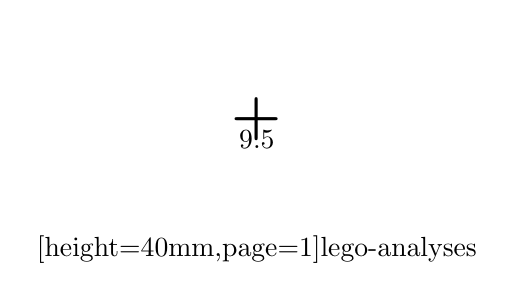
\begin{tikzpicture}
		\node (lego) at (0,-1.7) {\pic[height=40mm,page=1]{lego-analyses}};
		\node (lego) at (0,-.05) {\huge \textbf{+}};
		\node (lego) at (0,1) {\footnotesize\featureDiagramLego};
		\node at (0,-.3) {\mglass{9.5}};
	\end{tikzpicture}
}

\newcommand{\summaryproductbased}{
	\centering\pic[width=.8\linewidth,page=9]{lego-analyses}
	\mynote{Product-Based Strategy}{
		\begin{itemize}
			\item analyze individual \emph{products}
			\item[+] sound, complete
			\item[+] uses off-the-shelf generator\,$\gamma$ and analysis\,$\alpha$
			\item[--] redundant effort
			\item[--] does not scale well
		\end{itemize}
	}
}

\newcommand{\summaryfeaturebased}{
	\centering\pic[width=.8\linewidth,page=6]{lego-analyses}
	\mynote{Feature-Based Strategy}{
		\begin{itemize}
			\item analyze individual \emph{features}
			\item[+] sound, efficient
			\item[--] analysis $\alpha$ requires features with interfaces
			\item[--] incomplete: misses all feature interactions
		\end{itemize}
	}
}

\newcommand{\summaryfamilybased}{
	\centering\scalebox{.5}{\familybasedlego}
	\mynote{Family-Based Strategy}{
		\begin{itemize}
			\item analyze the \emph{product line}
			\item[+] sound, complete, efficient
			\item[--] requires careful, hand-crafted analysis $\alpha$
		\end{itemize}
	}
}

\subsection{Recap: Quality Assurance}

\begin{frame}{\myframetitle\ \mytitlesource{\ludewiglichter}}
	\begin{mycolumns}[widths={45},animation=none]
		\uncover<2->{\mynote{}{
			\begin{itemize}
				\item last lecture:\\
					how to \emph{avoid} variability bugs (esp. feature interactions)
				\uncover<4->{\item this + next lecture:\\
					how to \emph{find} variability bugs}
			\end{itemize}
		}}
	\mynextcolumn
		\only<1|handout:0>{\includegraphics[height=\textheightwithtitle,page=1]{quality-assurance}}%
		\only<2|handout:0>{\includegraphics[height=\textheightwithtitle,page=2]{quality-assurance}}%
		\only<3|handout:0>{\includegraphics[height=\textheightwithtitle,page=3]{quality-assurance}}%
		\only<4|handout:0>{\includegraphics[height=\textheightwithtitle,page=4]{quality-assurance}}%
		\only<5|handout:1>{\includegraphics[height=\textheightwithtitle,page=5]{quality-assurance}}%
		\only<6|handout:0>{\includegraphics[height=\textheightwithtitle,page=6]{quality-assurance}}%
	\end{mycolumns}
\end{frame}

\widexkcdframe{1700}

\subsection{Automated Analysis of Product Lines}

\begin{frame}{\myframetitle}
	\begin{mycolumns}[t,widths={47}]
		\mynote{Typical Program Analyses}{
			\leftandright{
				\begin{itemize}
					\item code metrics
					\item type checking
					\item theorem proving
					\item data-flow analysis
					\item performance analysis
					\item \ldots
				\end{itemize}
			}{
				\hspace*{10mm}\mglass{3}
			}
		}
		\mydefinition{What is a Program Analysis?}{
			\begin{itemize}
				\item analyzes properties of a \emph{program} (e.g., correctness, performance, and safety)
				\item can be used to automatically find bugs, bottlenecks, and other \emph{vulnerabilities}
			\end{itemize}
		}
		\mynextcolumn
		\myexample{Asking Questions About Product Lines}{
			\begin{itemize}
				\item Which product has the most lines of code? \mysource{\href{https://dl.acm.org/doi/10.1145/3307630.3342384}{ref}}
				\item Which products have type errors? \mysource{\href{https://dl.acm.org/doi/10.1145/1868688.1868693}{ref}}
				\item Which products violate specifications? \mysource{\href{https://dl.acm.org/doi/10.1145/2371401.2371404}{ref}}
				\item Which products have unsafe data flows? \mysource{\href{https://dl.acm.org/doi/10.1145/2499370.2491976}{ref}}
				\item Which is the fastest product? \mysource{\href{https://link.springer.com/article/10.1007/s10515-020-00273-8}{ref}}\\
					Which product has the smallest binary? \mysource{\href{https://dl.acm.org/doi/10.1145/3546932.3546997}{ref}}
				\item \ldots
			\end{itemize}
		}
		\mydefinition{What is a Product-Line Analysis?}{
			\begin{itemize}
				\item analyzes properties of an entire \emph{product line}
				\item can be roughly classified by its \emph{strategy}:
				\begin{itemize}
					\item product-based
					\item feature-based
					\item family-based
				\end{itemize}
			\end{itemize}
		}
	\end{mycolumns}
\end{frame}

\subsection{Product-Based Strategies} % refs missing in whole part!

\begin{frame}{\myframetitle}
	\begin{mycolumns}
		\mydefinition{Intuition}{
			\begin{itemize}
				\item to analyze the product line, just analyze \emph{each product}
				\begin{itemize}
					\item individually
					\item in isolation
					\item possibly in parallel
				\end{itemize}
				\item e.g., compile and verify each product
			\end{itemize}
		}
		\myexampletight{}{\centering\featureDiagramLego\\$Helmet \pimplies \pnot Phone$}
	\mynextcolumn
		\pic[width=\linewidth,page=9]{lego-analyses}
	\end{mycolumns}
\end{frame}

\begin{frame}{\myframetitle}
	\begin{mycolumns}
		\mydefinition{Algorithm}{
			\begin{algorithmic}
				\Require a product line $pl$; algorithms $\gamma$, $\alpha$, $\sigma$
				\State $C \gets AllSAT(\phi(FM_{pl}))$ \Comment{{\small enumerate valid config's}}
				\State $results \gets []$
				\ForAll{$S \in C$} \Comment{{\small for each valid config}}
				\State $p \gets \gamma(S)$ \Comment{{\small generate product}}
				\State $results \pluseq \alpha(p)$ \Comment{{\small add analysis result}}
				\EndFor
				\State \Return $\sigma(results)$
			\end{algorithmic}
		}
		\mynote{}{
			\begin{itemize}
				\item $\gamma$ \emph{generates} (e.g., compiles) products (e.g., \texttt{make}, \texttt{gradle}, \texttt{FeatureHouse}, \texttt{npm}, \ldots)
				\item $\alpha$ \emph{analyzes} the product (e.g., run verifier)
				\item $\sigma$ \emph{summarizes} the results (e.g., each individual call to $\alpha$ must succeed)
			\end{itemize}
		}
	\mynextcolumn
		\myexampletight{}{
			\begin{center}
				\small\featureDiagramConfigurableDatabase
			\end{center}
		}
		\myexample{}{
			\footnotesize
			\leftandright{
				$\sigma([\alpha(\gamma(\{C,G,W\}))$\\
				$~~~~\alpha(\gamma(\{C,P,W\}))$\\
				$~~~~\alpha(\gamma(\{C,G,P,W\}))$\\
				$~~~~\alpha(\gamma(\{C,D,W\}))$\\
				$~~~~\alpha(\gamma(\{C,G,D,W\}))$\\
				$~~~~\alpha(\gamma(\{C,P,D,W\}))$\\
				$~~~~\alpha(\gamma(\{C,G,P,D,W\}))$\\
				$~~~~\alpha(\gamma(\{C,P,T,W\}))$\\
				$~~~~\alpha(\gamma(\{C,G,P,T,W\}))$\\
				$~~~~\alpha(\gamma(\{C,D,T,W\}))$\\
				$~~~~\alpha(\gamma(\{C,G,D,T,W\}))$\\
				$~~~~\alpha(\gamma(\{C,P,D,T,W\}))$\\
				$~~~~\alpha(\gamma(\{C,G,P,D,T,W\}))$
			}{
				$\alpha(\gamma(\{C,G,L\}))$\\
				$\alpha(\gamma(\{C,P,L\}))$\\
				$\alpha(\gamma(\{C,G,P,L\}))$\\
				$\alpha(\gamma(\{C,D,L\}))$\\
				$\alpha(\gamma(\{C,G,D,L\}))$\\
				$\alpha(\gamma(\{C,P,D,L\}))$\\
				$\alpha(\gamma(\{C,G,P,D,L\}))$\\
				$\alpha(\gamma(\{C,P,T,L\}))$\\
				$\alpha(\gamma(\{C,G,P,T,L\}))$\\
				$\alpha(\gamma(\{C,D,T,L\}))$\\
				$\alpha(\gamma(\{C,G,D,T,L\}))$\\
				$\alpha(\gamma(\{C,P,D,T,L\}))$\\
				$\alpha(\gamma(\{C,G,P,D,T,L\}))])$
			}
		}
	\end{mycolumns}
\end{frame}

\begin{frame}{Classification of Strategies}
	\begin{mycolumns}[t,columns=3,animation=none]
		\summaryproductbased
	\mynextcolumn
	\mynextcolumn
	\end{mycolumns}
\end{frame}

\subsection{Feature-Based Strategies}

\begin{frame}{\myframetitle}
	\begin{mycolumns}
		\mydefinition{Intuition}{
			\begin{itemize}
				\item to analyze the product line, just analyze \emph{each feature} individually
				\item ignore all relations to other features
				\item e.g., compile and verify each component\\
				$\Rightarrow$ requires \emph{interfaces between features} (components, services, plug-ins) % todo: rename lecture 6 accordingly?
			\end{itemize}
		}
		\myexampletight{}{\centering\featureDiagramLego\\$Helmet \pimplies \pnot Phone$}
	\mynextcolumn
		\pic[width=\linewidth,page=6]{lego-analyses}
	\end{mycolumns}
\end{frame}

\begin{frame}{\myframetitle}
	\begin{mycolumns}
		\mydefinition{Algorithm}{
			\begin{algorithmic}
				\Require a product line $pl$; algorithms $\alpha$, $\sigma$
				\State $results \gets []$
				\ForAll{$f \in F_{pl}$} \Comment{{\small for each feature}}
				\State $results \pluseq \alpha(f)$ \Comment{{\small add analysis result}}
				\EndFor
				\State \Return $\sigma(results)$
			\end{algorithmic}
		}
		\mynote{}{
			\begin{itemize}
				\item $\alpha$ \emph{analyzes} the feature (e.g., compiles and verifies the component)
				\item $\sigma$ \emph{summarizes} the results (see product-based)
			\end{itemize}
		}
	\mynextcolumn
		\myexampletight{}{
			\begin{center}
				\small\featureDiagramConfigurableDatabase
			\end{center}
		}
		\myexample{}{
			\vspace*{-4ex}
			\small
			\begin{align*}
				\sigma([&\alpha(\gamma(C)) \text{ -- e.g., compile and verify base code}\\
				&\alpha(\gamma(G)) \text{ -- e.g., compile and verify feature Get}\\
				&\alpha(\gamma(P)) \text{ -- \ldots}\\
				&\alpha(\gamma(D))\\
				&\alpha(\gamma(T))\\
				&\alpha(\gamma(W))\\
				&\alpha(\gamma(L))])
			\end{align*}
		}
	\end{mycolumns}
\end{frame}

\begin{frame}{Classification of Strategies}
	\begin{mycolumns}[t,columns=3,animation=none]
		\summaryproductbased
	\mynextcolumn
		\summaryfeaturebased
	\mynextcolumn
	\end{mycolumns}
\end{frame}

\subsection{Family-Based Strategies}

\begin{frame}{\myframetitle}
	\begin{mycolumns}
		\mydefinition{Intuition}{
			\begin{itemize}
				\item analyze the product line (or \emph{family}) as a whole
				\item requirement: the analysis should give the same result as a product-based analysis
				\item makes use of the feature model and artifacts
				\item analysis is \emph{hand-crafted}, no generic algorithm\\
				$\Rightarrow$ typically: reduction to SAT problems
			\end{itemize}
		}
		\myexample{Today's Examples}{
			\begin{itemize}
				\item analyzing \emph{feature mappings}
				\item analyzing \emph{variable code}
			\end{itemize}
			$\Rightarrow$ here: only for \emph{conditional compilation}
		}
	\mynextcolumn
		\centering\familybasedlego
	\end{mycolumns}
\end{frame}

\subsection{Classification of Strategies}

\begin{frame}{\myframetitle}
	\begin{mycolumns}[t,columns=3,animation=none]
		\summaryproductbased
	\mynextcolumn
		\summaryfeaturebased
	\mynextcolumn
		\summaryfamilybased
	\end{mycolumns}
\end{frame}
\lessonslearned{
	\item product-line analyses are needed for quality assurance
	\item \emph{product-based}: simple, but does not scale
	\item \emph{feature-based}: fairly simple, but misses interactions
	\item \emph{family-based}: efficient, but most complex
}{
	\item \fospl\mychapter{10}
	\item \analysisstrategies
}{
	Can you imagine other analysis strategies than product-based, feature-based, and family-based?
	How could such strategies look like?
}

\section{Analyzing Feature Mappings}

\newcommand{\notleftright}{\mathrel{\ooalign{$\Leftrightarrow$\cr\hidewidth$/$\hidewidth}}}

\subsection{The Use of Feature-Mapping Analyses}

\begin{frame}{\myframetitle}
	\begin{mycolumns}[widths={45,55}]
		\mynote{Recap: A Typical Product Line}{
			\begin{itemize}
				\item embedded or systems programming (e.g., Linux)
				\item implemented with conditional compilation
				\begin{itemize}
					\item build systems (e.g., KBuild)
					\item preprocessors (e.g., CPP)
				\end{itemize}
				\item feature traceability only implicit\\
					$\Rightarrow$ there is code scattering and tangling
			\end{itemize}
		}
		\mydefinition{Recap: Feature Mapping}{
			\begin{itemize}
				\item \todots
			\end{itemize}
		}
		\mynextcolumn
		\myexample{Asking Questions About the Feature Mapping}{
			\begin{itemize}
				\item Are there contradictory or unnecessary preprocessor annotations in the code?
				\item Is the code even included in any product?
				\item If so, in how many products is the code included?
				\item \ldots
			\end{itemize}
		}
		\myexampletight{Running Example}{
			\centering
			\featureDiagram{Graph,concrete[Node,concrete,mandatory[Labeled,concrete,optional][Colored,concrete,optional]][Edge,concrete,mandatory[Directed,concrete,optional][Undirected,concrete,optional][Hyper,concrete,optional]]}
			$\pnot (Directed \pand Undirected)$\\
			$Hyper \pimplies Undirected$\\
			$Directed \notleftright (Undirected \pand Hyper)$\\
			\todo{revise CTCs}
		}
	\end{mycolumns}
\end{frame}

% mit quadranten starten
%wir gucken uns jetzt Source Code an (evtl. linke zwei (VL 4, Problem Space) + rechte zwei Quadranten (VL 10+, Solution Space))
% wechselwirkung zw. sol und problem space (mapping+FM)

\subsection{Presence Conditions}

\begin{frame}[fragile]{\myframetitle}
	\begin{mycolumns}[columns=3,widths={40,23,37},animation=none]
		\mydefinition{Presence Condition}{
			A \emph{presence condition (PC)} for a code location (i.e., a line/chunk/file) is a formula that describes the circumstances under which the code location is included in a product.
		}
		\mynote{}{
			\begin{itemize}
				\item useful for implementation techniques with code scattering and tangling
				\item e.g., build systems (file PCs) or preprocessors (line/chunk PCs)
				\item here: C preprocessor
			\end{itemize}
		}
	\mynextcolumn
		\myexampletight{Presence Conditions}{
			\small
			\begin{flushright}
				$\top$\\
				$Labeled$\\
				$Labeled$\\
				$Labeled$\\
				$Colored$\\
				$Colored$\\
				$Colored$\\
				$\top$\\
				$\top$\\
				$\top$\\
				$Directed$\\
				$Directed$\\
				$\pnot Dir \pand Hyper$\\
				$\pnot Dir \pand Hy \pand Un$\\
				$\pnot Dir \pand Hy \pand Un$\\
				$\pnot Dir \pand Hy \pand \pnot Un \pand Dir$\\
				$\pnot Dir \pand Hy \pand \pnot Un \pand Dir$\\
				$\pnot Dir \pand Hy \pand \pnot Un \pand Dir$\\
				$\pnot Dir \pand \pnot Hy \pand \pnot Dir$\\
				$\pnot Dir \pand \pnot Hy \pand \pnot Dir$\\
				$\pnot Dir \pand \pnot Hy \pand \pnot Dir$\\
				$\top$
			\end{flushright}
		}
	\mynextcolumn
		\begin{cpptight}[basicstyle=\small]{Product-Line Implementation}
class Node {
#ifdef LABELED
	string label;
#endif
#ifdef COLORED
	string color;
#endif
};

class Edge {
#ifdef DIRECTED
	Node fromNode, toNode;
#elifdef HYPER
#ifdef UNDIRECTED
	set<Node> nodeSet;
#elifdef DIRECTED
	map<Node, set<Node>> nodeMap;
#endif
#elifndef DIRECTED
#error Unsupported edge type.
#endif
};
		\end{cpptight}
	\end{mycolumns}
\end{frame}

\subsection{Detecting Dead Code}

\begin{frame}[fragile]{\myframetitle}
	\begin{mycolumns}[columns=3,widths={40,23,37},animation=none]
		\mydefinition{Dead Code}{
			A line/chunk/file of code is \emph{dead} when

			\begin{itemize}
				\item no product includes it.
				\item or, equivalently:\\
					its presence condition $PC$ is contradictory (i.e., $PC \mequals \bot$).
			\end{itemize}
		}
		\mynote{}{
			calculated by querying a \emph{satisfiability solver} whether $PC$ is not satisfiable (i.e., $\pnot SAT(PC)$)
		}
		\mynote{What causes dead code?}{
			\begin{itemize}
				\item confusion due to nested \texttt{\#ifdef}
				\item domain modeling mistakes
				\item can be intended! \mysource{\href{https://dl.acm.org/doi/10.1145/3442391.3442406}{Hentze~et~al.~2021}}
			\end{itemize}
		}
	\mynextcolumn
		\myexampletight{Presence Conditions}{
			\small\vspace*{-1.7ex}
			\begin{flushright}
				{\color{gray}$\top$}\\
				{\color{gray}$Labeled$}\\
				{\color{gray}$Labeled$}\\
				{\color{gray}$Labeled$}\\
				{\color{gray}$Colored$}\\
				{\color{gray}$Colored$}\\
				{\color{gray}$Colored$}\\
				{\color{gray}$\top$}\\
				{\color{gray}$\top$}\\
				{\color{gray}$\top$}\\
				{\color{red}$Directed$}\\
				{\color{gray}$Directed$}\\
				{\color{red}$\pnot Dir \pand Hyper$}\\
				{\color{gray}$\pnot Dir \pand Hy \pand Un$}\\
				{\color{gray}$\pnot Dir \pand Hy \pand Un$}\\
				{\color{red}$\pnot Dir \pand Hy \pand \pnot Un \pand Dir$}\\
				{\color{red}$\pnot Dir \pand Hy \pand \pnot Un \pand Dir$}\\
				{\color{red}$\pnot Dir \pand Hy \pand \pnot Un \pand Dir$}\\
				{\color{gray}$\pnot Dir \pand \pnot Hy \pand \pnot Dir$}\\
				{\color{gray}$\pnot Dir \pand \pnot Hy \pand \pnot Dir$}\\
				{\color{gray}$\pnot Dir \pand \pnot Hy \pand \pnot Dir$}\\
				{\color{gray}$\top$}
			\end{flushright}
		}
	\mynextcolumn
		\begin{cpptight}[basicstyle=\small]{Product-Line Implementation}
class Node {
#ifdef LABELED
	string label;
#endif
#ifdef COLORED
	string color;
#endif
};

class Edge {
#ifdef DIRECTED
	Node fromNode, toNode;
#elifdef HYPER
#ifdef UNDIRECTED
	set<Node> nodeSet;
#elifdef DIRECTED
	@map<Node, set<Node>> nodeMap;@
#endif
#elifndef DIRECTED
#error Unsupported edge type.
#endif
};
		\end{cpptight}
	\end{mycolumns}
\end{frame}

% dead code paper (tartler beteiligt, erlangen evtl., TDS+:ATC14/EuroSys11) in linux? technik zum code auskommentieren, nicht alles ist ungewollt

\subsection{Detecting Superfluous Annotations}

\begin{frame}[fragile]{\myframetitle}
	\begin{mycolumns}[columns=3,widths={40,23,37},animation=none]
		\mydefinition{Superfluous Annotation}{
			An annotation is (partly) \emph{superfluous}

			\begin{itemize}
				\item when it can be omitted (or simplified) without consequences.
				\item or, equivalently:\\
					its presence condition $PC$ is contradictory (i.e., $PC \mequals \bot$).
			\end{itemize}
		}
		\mynote{}{
			calculated by querying a \emph{satisfiability solver} whether $PC$ is not satisfiable (i.e., $\pnot SAT(PC)$)
		}
		\mynote{What causes dead code?}{
			\begin{itemize}
				\item confusion due to nested \texttt{\#ifdef}
				\item domain modeling mistakes
				\item can be intended! \mysource{\href{https://dl.acm.org/doi/10.1145/3442391.3442406}{Hentze~et~al.~2021}}
			\end{itemize}
		}
	\mynextcolumn
		\myexampletight{Presence Conditions}{
			\small\vspace*{-1.7ex}
			\begin{flushright}
				{\color{gray}$\top$}\\
				{\color{gray}$Labeled$}\\
				{\color{gray}$Labeled$}\\
				{\color{gray}$Labeled$}\\
				{\color{gray}$Colored$}\\
				{\color{gray}$Colored$}\\
				{\color{gray}$Colored$}\\
				{\color{gray}$\top$}\\
				{\color{gray}$\top$}\\
				{\color{gray}$\top$}\\
				{\color{gray}$Directed$}\\
				{\color{gray}$Directed$}\\
				{\color{gray}$\pnot Dir \pand Hyper$}\\
				{\color{gray}$\pnot Dir \pand Hy \pand Un$}\\
				{\color{gray}$\pnot Dir \pand Hy \pand Un$}\\
				{\color{gray}$\pnot Dir \pand Hy \pand \pnot Un \pand Dir$}\\
				{\color{gray}$\pnot Dir \pand Hy \pand \pnot Un \pand Dir$}\\
				{\color{gray}$\pnot Dir \pand Hy \pand \pnot Un \pand Dir$}\\
				{\color{red}$\pnot Dir \pand \pnot Hy \pand \pnot Dir$}\\
				{\color{red}$\pnot Dir \pand \pnot Hy \pand \pnot Dir$}\\
				{\color{red}$\pnot Dir \pand \pnot Hy \pand \pnot Dir$}\\
				{\color{gray}$\top$}
			\end{flushright}
		}
	\mynextcolumn
		\begin{cpptight}[basicstyle=\small]{Product-Line Implementation}
class Node {
#ifdef LABELED
	string label;
#endif
#ifdef COLORED
	string color;
#endif
};

class Edge {
#ifdef DIRECTED
	Node fromNode, toNode;
#elifdef HYPER
#ifdef UNDIRECTED
	set<Node> nodeSet;
#elifdef DIRECTED
	map<Node, set<Node>> nodeMap;
#endif
#elifndef @DIRECTED@
#error Unsupported edge type.
#endif
};
		\end{cpptight}
	\end{mycolumns}
\end{frame}

\subsection{Considering the Feature Model}

%bezug auf FM-analyse
% + variability smells erwähnen

% show how linux in lecture 4+5 relates to problem space (kconfig)/mapping (kbuild)/solution space (cpp)
% maybe consider FM + KBuild? the whole chain?

\begin{frame}{\myframetitle}
	\begin{mycolumns}
	\mynextcolumn
	\end{mycolumns}
\end{frame}

\subsection{Feature-Mapping Analyses in FeatureIDE}

\begin{frame}{\myframetitle}
	\begin{mycolumns}
		\href{https://youtu.be/jVe7f32mLCQ?t=125}{demo video available} (minute 3 and 4): dead code block, superfluous annotations, generation of all products, error propagation, unit testing
	\mynextcolumn
		\mynote{Discussion}{
			\begin{itemize}
				\item only the feature mapping is analyzed, the source code is ignored
				\begin{itemize}
					\item pro: simple, language-independent
					\item con: can only find simple anomalies
				\end{itemize}
			\end{itemize}
		}
	\end{mycolumns}
\end{frame}

\lessonslearned{
	\item feature-mapping analyses alleviate the impact of code scattering and tangling
	\item they are usually not necessary when there is good feature traceability
	\item they cannot detect bugs in the actual code
}{
	\item \fospl\mychapter{10}
}{
	Above, we assumed that we know all presence conditions already.
	How can we automatically extract presence conditions from code that uses the C preprocessor?
	What problems might occur?
	% - there might be #includes that contain macro definitions
	% - there might be macros to be expanded, which can get complex quickly
	% - it is not always trivial to distinguish feature macros from compiler- or system-specific macros
	% - there is #undef (or re-#define), which opens another can of worms
	% see works on TypeChef (C. Kästner), SuperC (P. Gazillo), FeatureCoPP (K. Ludwig), PCLocator (E. Kuiter)
}

\section{Analyzing Variable Code}
% Code + Mapping + FM

\subsection{One or two of the following:}

\subsection{Type Checking} % Hauptfokus

%\subsection{Static Analysis} - ist mapping

%\subsection{Model Checking}

\subsection{Theorem Proving / Variability Encoding}
%variability encoding, aber nur auf einer Folie
% #ifdef in if überführen + welche Tools kann man jetzt easy anwenden?
\lessonslearned{
	\item with family-based analyses of variable code, we can analyze (non-)functional properties of all products at once
	\item type checking all products at once is possible for product lines up to medium size
	\item for huge product lines (e.g., Linux), it is infeasible
}{
	\item \fospl\mychapter{10}
	\item \typechef
}{
	Suppose you have a preprocessor-based product line (with \texttt{\#ifdef}'s).
	If you could turn it into a single, large runtime-variable product (with \texttt{if}'s), you could use an off-the-shelf compiler to find any type error in any product.

	Is this possible? What problems might occur?
	\mysource{\sugarc}
}

\faq{
	\item How to find variability bugs?
	\item What is a program analysis? What are examples?
	\item What is a product-line analysis?
	\item What are principal strategies to analyze product lines? What are (dis-)advantages?
	\item Given a specific algorithm, classify its analysis strategy!
}{
	\item How to analyze feature mappings?
	\item What are potential problems in feature mappings?
	\item What are presence conditions, dead code, superfluous annotations?
	\item Shall we incorporate the feature model when analyzing feature mappings?
	\item Shall product-line analyses analyze problem and solution space separately?
	\item What is special when analyzing the feature mapping of feature modules?
	\item What are limitations of analyzing feature mappings?
	\item Given CPP source code, determine its presence conditions, dead code, and superfluous annotations!
}{
	\item What are (examples of) type errors?
	\item Why are type errors challenging to detect in product lines?
	\item What is a type-safe product line, reachability condition, conflict condition?
	\item How does the analysis complexity differ for real-world product lines?
	\item What are analyses for problem and solution space?
	\item Give examples for easy and difficult product lines in terms of analysis effort!
}

\mode<beamer>{
	\begin{frame}{\inserttitle}
		\lectureseriesoverview
	\end{frame}

	\contentoverview
}


% TODO L11 PRODUCT-LINE TESTING

\ifuniversity{recording}{\date{June 21, 2023}\setpicture[200]{may23-south}\setcopyright{}}
\ifuniversity{ulm}{\date{July 6, 2023}\setpicture[200]{may23-south}}
\ifuniversity{magdeburg}{\setpicture[110]{ovgu-winter5}\setcopyright{Photo: Hannah Theile (OVGU)}}
\ifuniversity{paderborn}{\date{June 26, 2024}\setpicture[50]{pressimage7}}

\author{Thomas Thüm, Sebastian Krieter, Timo Kehrer, Elias Kuiter}
\lecture{Product-Line Testing}{testing}

\begin{frame}{Recap: Quality Assurance \deutschertitel{Qualitätssicherung} \mytitlesource{\ludewiglichter}}
	\begin{fancycolumns}[widths={60},animation=none]
		%\only<1|handout:0>{\includegraphics[width=\linewidth,page=1]{quality-assurance}}%
		\only<1|handout:0>{\picDark[width=\linewidth,page=8]{quality-assurance}}%
		\only<2|handout:0>{\picDark[width=\linewidth,page=3]{quality-assurance}}%
		\only<3|handout:0>{\picDark[width=\linewidth,page=4]{quality-assurance}}%
		\only<4|handout:1>{\picDark[width=\linewidth,page=5]{quality-assurance}}%
		\only<5-|handout:0>{\picDark[width=\linewidth,page=7]{quality-assurance}}%
	\nextcolumn
		\begin{note}{Lectures on Quality Assurance}
			how to \emph{avoid} variability bugs\\(esp. feature interactions) \ldots
			\begin{itemize}
				\item<+-> with processes\mysource{\lectureprocess}\\(e.g., domain scoping)
				\item<+-> with guidelines\mysource{\lectureinteractions}
			\end{itemize}
			\visible<3->{how to \emph{find} variability bugs \ldots}
			\begin{itemize}
				\item<+-> \emph{statically}\mysource{\lectureanalyses}
				\item<+-> \emph{dynamically}\mysource{\lecturetesting}\\
				\begin{itemize}
					\item<+-> challenges of product-line testing in Part~\parta
					\item<+-> black-box testing in Part~\partb
					\item<+-> white-box testing in Part~\partc
				\end{itemize}
			\end{itemize}
		\end{note}
	\end{fancycolumns}
\end{frame}

% TODO add xkcd from SWT? \widexkcd{974} % salt 12s

\section{Challenges of Product-Line Testing}
% TODO \section{Product-Line Testing in Practice} practice part still missing
% TODO famous example for a product line failure?

\subsection{Recap: Software Testing}
\begin{frame}{\myframetitle{}}
	\begin{fancycolumns}
		\uncover<1->{
			\begin{definition}{Software Testing \mysource{\sommerville}}
				\mycite{Testing is intended to show that a program does what it is intended to do and to discover program defects before it is put into use.}
			\end{definition}
		}
		\uncover<2->{
			\begin{definition}{Validation Testing \mysource{\sommerville}}
				\mycite{Demonstrate to the developer and the customer that the software meets its requirements.}
			\end{definition}
		}
		\uncover<3->{
			\begin{definition}{Defect Testing \mysource{\sommerville}}
				\mycite{Find inputs or input sequences where the behavior of the software is incorrect, undesirable, or does not conform to its specification.}
			\end{definition}
		}
	\nextcolumn
		\uncover<4->{
			\begin{note}{Stages of Testing \mysource{\sommerville}}
				\begin{itemize}
					\setlength\itemsep{.1em}
					\item[1.] \mycite{\emph{Development testing}, where the system is tested during development to discover
					bugs and defects}
					\item[2.] \mycite{\emph{Release testing}, where a separate testing team tests a complete version of the
					system before it is released to users}
					\item[3.] \mycite{\emph{User testing}, where users or potential users of a system test the system in their
					own environment}
				\end{itemize}
			\end{note}
		}
		\uncover<5->{
			\begin{note}{Manual vs Automated Testing \mysource{\sommerville}}
				\mycite{In \emph{manual testing}, a tester runs the program with some test data and
				compares the results to their expectations. [...] In \emph{automated testing}, the tests are encoded in a program that is run each time the system under development is to be tested.}
			\end{note}
		}
	\end{fancycolumns}
\end{frame}

\subsection{Test-Case Design in Single-System Engineering}
\begin{frame}{Recap: Test-Case Design \deutschertitel{Testfallentwurf}}
	\begin{fancycolumns}
		\begin{definition}{Test Case \mysource{\ludewiglichter}}
			In a test, a number of test cases are executed, whereas each test case consists \emph{input values} for a single execution and \emph{expected outputs}. An \emph{exhaustive test} refers a test in which the test cases exercise all the possible inputs.
		\end{definition}
		\pause
		\begin{definition}{Systematic Test \mysource{\ludewiglichter}}
			A systematic test is a test, in which
			\begin{itemize}
				\setlength\itemsep{.1em}
				\item[1.] the \emph{setup} is defined,
				\item[2.] the \emph{inputs} are chosen systematically,
				\item[3.] the \emph{results} are documented and evaluated by criteria being defined prior to the test. 
			\end{itemize}
		\end{definition}
	\nextcolumn
		\pause
		\begin{note}{Goal \mysource{\ludewiglichter}}%
			Detect a large number of failures with a low number of test cases. A test case (execution) is \emph{positive}, if it detects a failure, and \emph{successful} if it detects an unknown failure.
		\end{note}
		\pause
		\begin{definition}{An ideal test case is \ldots \mysource{\ludewiglichter}}
			\begin{itemize}
				\setlength\itemsep{.1em}
				\item representative: represents a large number of feasible test cases
				\item failure sensitive: has a high probability to detect a failure
				\item non-redundant: does not check what other test cases already check
			\end{itemize}
		\end{definition}
	\end{fancycolumns}
\end{frame}

% TODO recap analysis strategies for product lines and discuss why feature based and family based is typically not feasible for testing

\subsection{Testing All Configurations}
\begin{frame}{\myframetitle{}}
	\begin{fancycolumns}
		\centering\featureDiagramConfigurableDatabase
		
		\begin{example}{Recap: 26 Valid Configurations\mysource{\lecturemodeling}}
			\footnotesize
			\begin{fancycolumns}[animation=none]
				$\{C,G,W\}$\\
				$\{C,P,W\}$\\
				$\{C,G,P,W\}$\\
				$\{C,D,W\}$\\
				$\{C,G,D,W\}$\\
				$\{C,P,D,W\}$\\
				$\{C,G,P,D,W\}$\\
				$\{C,P,T,W\}$\\
				$\{C,G,P,T,W\}$\\
				$\{C,D,T,W\}$\\
				$\{C,G,D,T,W\}$\\
				$\{C,P,D,T,W\}$\\
				$\{C,G,P,D,T,W\}$
			\nextcolumn
				$\{C,G,L\}$\\
				$\{C,P,L\}$\\
				$\{C,G,P,L\}$\\
				$\{C,D,L\}$\\
				$\{C,G,D,L\}$\\
				$\{C,P,D,L\}$\\
				$\{C,G,P,D,L\}$\\
				$\{C,P,T,L\}$\\
				$\{C,G,P,T,L\}$\\
				$\{C,D,T,L\}$\\
				$\{C,G,D,T,L\}$\\
				$\{C,P,D,T,L\}$\\
				$\{C,G,P,D,T,L\}$
			\end{fancycolumns}
		\end{example}
	\nextcolumn
		\vspace{-7mm}
		\pause
		\begin{note}{Discussion}
			\begin{itemize}
				\setlength\itemsep{.5em}
				\item only feasible for \emph{small} product lines\\(few valid configurations)
				\item redundant test effort
				\vspace*{1ex}
				\item large product lines: not feasible to generate and compile all configurations
				\begin{itemize}
					\item (some) large product lines: even number of valid configurations is unknown
				\end{itemize}
			\end{itemize}
		\end{note}
	\end{fancycolumns}
\end{frame}

\begin{frame}{Recap: Feature Model of the Linux Kernel}
	\vspace{1mm}~\hspace{-15mm}\href{https://dl.acm.org/doi/abs/10.1145/3382025.3414943}{\pic[width=1.2\linewidth,page=1,trim=100 510 100 170,clip]{2020/2020-SPLC-Thuem}}
\end{frame}

\begin{frame}{\myframetitle{}}
	\begin{fancycolumns}[widths={60}]
		\begin{exampletight}{Recap: Industrial Configuration Spaces\mysource{\lectureintroduction}}
			\centering\evaluatingsharpsatsolverslink{\pic[width=\linewidth,page=6,trim=50 210 320 440,clip]{2020/2020-VaMoS-Sundermann}}
		\end{exampletight}
		\uncover<3->{
			\begin{note}{}
				Why being complete on the configurations then?
			\end{note}
		}
	\nextcolumn
		\vspace{-7mm}
		\href{https://commons.wikimedia.org/wiki/File:Edsger_Wybe_Dijkstra.jpg}{\pic[width=\linewidth,trim=0 425 0 75,clip]{edsger-dijkstra}}
		\vspace{-7mm}
		
		\begin{note}{Edsger W. Dijkstra (1972)}
			\mycite{Program testing can be a very effective way to show the presence of bugs, but it is hopelessly inadequate for showing their absence.}\mysource{\thehumbleprogrammer}
		\end{note}
		% 1930-2002, ACM Turing Award winner
	\end{fancycolumns}
\end{frame}

\newcommand{\eemph}[1]{{\color{red}\textbf{#1}}}

\subsection{Testing One Configuration}
\begin{frame}[b]{\myframetitle{}}
	\begin{fancycolumns}[b]
		\centering\featureDiagramConfigurableDatabase
		
		\begin{example}{Recap: 26 Valid Configurations\mysource{\lecturemodeling}}
			\footnotesize
			\begin{fancycolumns}[animation=none]
				$\{C,G,W\}$\\
				$\{C,P,W\}$\\
				$\{C,G,P,W\}$\\
				$\{C,D,W\}$\\
				$\{C,G,D,W\}$\\
				$\{C,P,D,W\}$\\
				$\{C,G,P,D,W\}$\\
				$\{C,P,T,W\}$\\
				$\{C,G,P,T,W\}$\\
				$\{C,D,T,W\}$\\
				$\{C,G,D,T,W\}$\\
				$\{C,P,D,T,W\}$\\
				\emph{$\{C,G,P,D,T,W\}$}
			\nextcolumn
				$\{C,G,L\}$\\
				$\{C,P,L\}$\\
				$\{C,G,P,L\}$\\
				$\{C,D,L\}$\\
				$\{C,G,D,L\}$\\
				$\{C,P,D,L\}$\\
				$\{C,G,P,D,L\}$\\
				$\{C,P,T,L\}$\\
				$\{C,G,P,T,L\}$\\
				$\{C,D,T,L\}$\\
				$\{C,G,D,T,L\}$\\
				$\{C,P,D,T,L\}$\\
				$\{C,G,P,D,T,L\}$
			\end{fancycolumns}
		\end{example}
	\nextcolumn
		\pause\vspace{-10mm}
		\begin{note}{Discussion}
			\begin{itemize}
				\setlength\itemsep{.4em}
				\item applicable to large product lines
				\item no redundant test effort (from configurations)
				\item strategy in practice: all-yes-config (configuration with many features selected)
				\vspace*{1ex}
				\item often unfeasible to test all features wit a single configuration (e.g., \texttt{Windows} and \texttt{Linux})
				\item[$\Rightarrow$] unnoticed feature interactions\mysource{\lectureinteractions}
			\end{itemize}
		\end{note}
		\pause
		\begin{example}{What about interactions with missing features?}
			\centering\pic[width=.5\linewidth]{toast4}
		\end{example}
	\end{fancycolumns}
\end{frame}

\subsection{Sample-Based Testing}
\begin{frame}{\myframetitle{} \deutschertitel{Stichprobenbasiertes Testen}}
	\begin{fancycolumns}
		\begin{definition}{Intuition}
			\begin{itemize}
				\item to analyze the product line, just analyze \emph{some products}
				\item sample \deutsch{Stichprobe} refers to a subset of all valid configurations
				\item common technique to test a product line
				\item sample configurations chosen by experts, randomly, or systematically
			\end{itemize}
		\end{definition}
		\pause
		\begin{note}{Advantages and Challenges}
			\begin{itemize}
				\item[+] lower effort than testing all configurations
				\item[+] higher chance to detect defects than testing one configuration
				\item[--] how many configurations to test?\\which configurations to test?
			\end{itemize}
		\end{note}
	\nextcolumn
		\pause
		\pic[width=\linewidth,page=10]{lego-analyses}
	\end{fancycolumns}
\end{frame}

% TODO \subsection{Expert Knowledge in Sampling}

% TODO \subsection{Random Sampling}

% TODO probably too much content anyway: \subsection{Excursus: Uniform Random Sampling}

% TODO \subsection{Testing the Linux Kernel}
% allyesconfig

%\subsection{Automation in Product Sampling} ???

%\subsection{Missing: Test-Case Selection/Generation}
% What to test for those configurations? Variable unit tests? Avoid redundant testing?

% TODO how Linux is developed: patches on mailing list, only considered if not rejected by CI, what happens in CI


\lessonslearned{
	\item recap on software testing and test-case design
	\item testing all configurations
	\item testing one configuration
	\item sample-based testing
}{
	\item \samplingsurvey: overview on sampling literature
	\item \samplingsurveydatabase: database on sampling algorithms and evaluations
}{
	Recap on feature interactions: What are examples of interactions that cannot be detected statically (cf.\ \lectureanalyses) and could be missed when testing a single configuration only?
}

\section{Combinatorial Interaction Testing}
\subsection{Test-Case Design in Single-System Engineering}
\begin{frame}{Recap: Test-Case Design \deutschertitel{Testfallentwurf}}
	\leftorright{
		\uncover<1>{\mydefinition{Systematic Test \mysource{\ludewiglichter}}{A systematic test is a test, in which
			\begin{itemize}
				\setlength\itemsep{.1em}
				\item[1.] the setup is defined,
				\item[2.] the inputs are chosen systematically,
				\item[3.] the results are documented and evaluated by criteria being defined prior to the test. 
			\end{itemize}
		}{}}
		\uncover<2>{\mydefinition{Test Case \mysource{\ludewiglichter}}{In a test, a number of test cases are executed, whereas each test case consists \emph{input values} for a single execution and \emph{expected outputs}. An \emph{exhaustive test} refers a test in which the test cases exercise all the possible inputs.}{}}
	}{
		\mynote{Goal \mysource{\ludewiglichter}}{Detect a large number of failures with a low number of test cases. A test case (execution) is \emph{positive}, if it detects a failure, and \emph{successful} if it detects an unknown failure.}
		\mydefinition{An ideal test case is \ldots \mysource{\ludewiglichter}}{
			\begin{itemize}
				\setlength\itemsep{.1em}
				\item representative: represents a large number of feasible test cases
				\item failure sensitive: has a high probability to detect a failure
				\item non-redundant: does not check what other test cases already check
			\end{itemize}
		}{}
	}
\end{frame}

\begin{frame}{Recap: Black-Box Testing \deutschertitel{Funktionstest}}
	\begin{mycolumns}
		\begin{note}{Motivation \mysource{\ludewiglichter}}
			\begin{itemize}
				\setlength\itemsep{.1em}
				\item source code not always available (e.g., outsourced components, obfuscated code)
				%\item specific test cases derived from logical ones using arbitrary values
				%\item specification not incorporated so far (only for expected results)
				%\item invalid inputs not tested
				\item errors are not equally distributed
			\end{itemize}
		\end{note}
		\begin{definition}{Black-Box Testing \mysource{\ludewiglichter}}
			\begin{itemize}
				\setlength\itemsep{.1em}
				\item test-case design based on specification
				\item source code and its inner structure is ignored (assumed as a black-box)
			\end{itemize}
		\end{definition}
	\mynextcolumn
		\begin{note}{Sample Configuration $\neq$ Test Case}
			\begin{itemize}
				\item test case: concrete inputs and expected outputs for a program
				\item sample configuration: selection of features to derive the program
				\item both needed when testing product lines
				\item often confused in the literature
				\item test case derivation
					\begin{itemize}
						\item out of scope here % TODO add pointers to literature
						\item global tests (i.e., identical for all configurations)
						\item product-line implementation technique used to automatically derive configuration-specific tests \lectureprocess
					\end{itemize}
				\item on next slides: idea of black-box testing applied to derive sample configuration
			\end{itemize}
		\end{note}
	\end{mycolumns}
\end{frame}

\subsection{Pairwise Interaction Testing}
\begin{frame}{\myframetitle}
	\leftorright{
		\mydefinition{Pairwise Interaction Testing}{
			\begin{itemize}
				\setlength\itemsep{.5em}
				\item test a sample set $S \subseteq C$ of all valid configurations $C$ with pairwise coverage
				\item every pairwise interaction is covered by at least one configuration in the sample $S$
			\end{itemize}
		}
		\begin{example}{Configurations with the Interaction Get $\wedge$ Put}
			\footnotesize
			\leftandright{
				$\{C,G,W\}$\\
				$\{C,P,W\}$\\
				\emph{$\{C,G,P,W\}$}\\
				$\{C,D,W\}$\\
				$\{C,G,D,W\}$\\
				$\{C,P,D,W\}$\\
				\emph{$\{C,G,P,D,W\}$}\\
				$\{C,P,T,W\}$\\
				\emph{$\{C,G,P,T,W\}$}\\
				$\{C,D,T,W\}$\\
				$\{C,G,D,T,W\}$\\
				$\{C,P,D,T,W\}$\\
				\emph{$\{C,G,P,D,T,W\}$}
			}{
				$\{C,G,L\}$\\
				$\{C,P,L\}$\\
				\emph{$\{C,G,P,L\}$}\\
				$\{C,D,L\}$\\
				$\{C,G,D,L\}$\\
				$\{C,P,D,L\}$\\
				\emph{$\{C,G,P,D,L\}$}\\
				$\{C,P,T,L\}$\\
				\emph{$\{C,G,P,T,L\}$}\\
				$\{C,D,T,L\}$\\
				$\{C,G,D,T,L\}$\\
				$\{C,P,D,T,L\}$\\
				\emph{$\{C,G,P,D,T,L\}$}
			}
		\end{example}
	}{
		\mynote{Discussion}{
			\begin{itemize}
				\setlength\itemsep{.4em}
				\item applicable to large product lines
				\item reduced redundant effort compared to testing all configurations
				\item coverage guarantee (opposed to random configurations)
				\item still requires good test cases (program inputs)
				\item hard to compute small sample sets
			\end{itemize}
		}
		\mydefinition{Pairwise Interactions}{
			\begin{itemize}
				\setlength\itemsep{.5em}
				\item \emph{up-to} four interactions between $A$ and $B$
				\item both selected: $A \wedge B$
				\item one selected: $\neg A \wedge B$, $A \wedge \neg B$
				\item none selected: $\neg A \wedge \neg B$
			\end{itemize}
		}
	}
\end{frame}

\newcommand{\pair}[2]{$#1 \wedge #2$ & $#1 \wedge \neg #2$ & $\neg #1 \wedge #2$ & $\neg #1 \wedge \neg #2$\\}
\newcommand{\redandgray}[1]{\only<#1-| handout:#1->{\color{black}}\only<#1| handout:#1>{\color{blue}}}
\newcommand{\epair}[6]{
	{\redandgray{#3}$#1 \wedge #2$} & 
	{\redandgray{#4}$#1 \wedge \neg #2$} & 
	{\redandgray{#5}$\neg #1 \wedge #2$} & 
	{\redandgray{#6}$\neg #1 \wedge \neg #2$}\\
}

\begin{frame}{Pairwise Coverage}
	\leftorright{
		\centering\featureDiagramConfigurableDatabase

		\mydefinition{Interactions to Cover}{
			\begin{itemize}
				\setlength\itemsep{.5em}
				\item exclude invalid combinations (e.g., $W \wedge L$)
				\item exclude abstract features (e.g., $API$, $OS$)
				\item exclude features contained in every configuration (e.g., $C$)
			\end{itemize}
			% TODO \todo{add formal definitions based on \lecturemodeling}
		}
	}{
		\vspace{-10mm}
		\myexample{Pairwise Interactions}{
			\centering\footnotesize\color{lightgray}
			\begin{tabular}{llll}
				\epair{G}{P}{3}{2}{1}{6}
				\epair{G}{D}{2}{3}{1}{5}
				\epair{G}{T}{3}{2}{1}{5}
				\epair{G}{W}{4}{2}{1}{6}
				\epair{G}{L}{2}{4}{6}{1}
				\epair{P}{D}{1}{3}{2}{4}
				\epair{P}{T}{1}{5}{6}{2}
				\epair{P}{W}{1}{3}{4}{2}
				\epair{P}{L}{3}{1}{2}{4}
				\epair{D}{T}{1}{2}{3}{4}
				\epair{D}{W}{1}{2}{4}{3}
				\epair{D}{L}{2}{1}{3}{4}
				\epair{T}{W}{1}{3}{4}{2}
				\epair{T}{L}{3}{1}{2}{4}
				& {\redandgray{1}$W \wedge \neg L$} & {\redandgray{2}$\neg W \wedge L$} & \\
			\end{tabular} 
		}
		\myexample{Pairwise Coverage with Six Configurations}{
			\footnotesize\color{lightgray}
			{\redandgray{1}$\{C,P,D,T,W\}$}\\
			{\redandgray{2}$\{C,G,D,L\}$}\\
			{\redandgray{3}$\{C,G,P,T,L\}$}\\
			{\redandgray{4}$\{C,G,W\}$}\\
			{\redandgray{5}$\{C,P,W\}$}\\
			{\redandgray{6}$\{C,D,T,L\}$}\\
		}
	}
\end{frame}
% TODO use different colors for the different configurations (instead of separate handouts)

\subsection{T-Wise Interaction Testing}
\begin{frame}{\myframetitle}
	\begin{mycolumns}[widths={65}]
		\mydefinition{T-Wise Interaction Testing}{
			\begin{itemize}
				\setlength\itemsep{.5em}
				\item generalization of pairwise interaction testing
				\item t-wise coverage: every t-wise interaction is covered by at least one configuration in the sample
				\item t=1: every feature is selected and also deselected
				\item t=2: pairwise interaction coverage
				\item t=3: every combination of three features covered
			\end{itemize}
		}
	\mynextcolumn
		\begin{example}{{T=3 Interactions}}
			for the features $G$, $P$, and $D$:

			\leftandright{
				$G \wedge P \wedge D$\\
				$G \wedge P \wedge \neg D$\\
				$G \wedge \neg P \wedge D$\\
				$G \wedge \neg P \wedge \neg D$
			}{
				$\neg G \wedge P \wedge D$\\
				$\neg G \wedge P \wedge \neg D$\\
				$\neg G \wedge \neg P \wedge D$\\
				$\neg G \wedge \neg P \wedge \neg D$
			}
		\end{example}
	\end{mycolumns}
\end{frame}

\subsection{Algorithms for Combinatorial Interaction Testing}
\begin{frame}{\myframetitle}
	\begin{mycolumns}[widths={63}]
		\begin{definition}{A Greedy Algorithm}
			idea: select configuration that cover most of the missing interactions in each step
			\begin{enumerate}
				\item randomly choose first configuration (each covers one interaction of every line)
				\item find next optimal configuration
				\item repeat steps 2--3 until all interactions covered
			\end{enumerate}
		\end{definition}
		\pause
		\begin{note}{Challenges and Optimizations}
			\begin{itemize}
				\item non-deterministic: different sample for each run (cf.\ Step 1)
				\item starting with all-yes-config? covers more code
				\item Step 2: iterating over all valid configurations does not scale
				\item greedy strategy: optimal configuration in each step does not guarantee optimal sample
			\end{itemize}
		\end{note}
	\mynextcolumn
		\pause
		\begin{definition}{ICPL\mysource{\icpl}}
			\begin{itemize}
				\item widespread greedy algorithm
				\item maintains several partial configurations
				\item iterates over all interactions
				\item tries to integrate interaction into existing partial configuration
				\item create new partial configuration if not possible
				\item avoids extensive Step 2
				\item performance shown on next slides
			\end{itemize}
		\end{definition}
	\end{mycolumns}
\end{frame}

\subsection{Efficiency of Combinatorial Interaction Testing}
%\subsection{Combinatorial Interaction Testing with ICPL}
\begin{frame}{\myframetitle\ \mytitlesource{\icpl}}
	\leftorright{
		\myexampletight{Assumption: All Features are Optional}{
			\centering\footnotesize\featureDiagramEightOptionalFeatures
		}
		
		\myexampletight{Number of Configurations in Pairwise Sample}{
			\includegraphics[width=\linewidth,page=4]{cit-plots}
		}
	}{%
		\myexampletight{Assumption: All Features are Optional}{
			\centering\footnotesize\featureDiagramEightOptionalFeatures
		}
		
		\myexampletight{Number of Configurations in T-Wise Sample}{
			\includegraphics[width=\linewidth,page=5]{cit-plots}
		}
	}
\end{frame}

\begin{frame}{\myframetitle\ \mytitlesource{\icpl}}
	\leftorright{
		\myexampletight{Time in Minutes to Compute Sample}{
			\includegraphics[width=\linewidth,page=2]{cit-plots}

			\begin{itemize}
				\setlength\itemsep{.5em}
				\item about 9h for Linux
				\item 480 configuration in pairwise sample
			\end{itemize}
		}
	}{
		\myexampletight{Number of Configurations in Sample}{
			\includegraphics[width=\linewidth,page=3]{cit-plots}

			\begin{itemize}
				\setlength\itemsep{.5em}
				\item Linux kernel v2.6.28.6 (February 2009)
				\item 6,888 features
				\item 187,193 clauses in conjunctive normal form
			\end{itemize}
		}
	}
\end{frame}

% TODO distinguish testing efficiency and sampling efficiency

\subsection{Effectiveness of Combinatorial Interaction Testing}
\begin{frame}{\myframetitle}
	\leftorright{
		\myexampletight{Effectiveness of Interaction Testing \mysource{\href{https://ieeexplore.ieee.org/document/1321063}{Kuhn et al.\ 2004}}}{
			\includegraphics[width=\linewidth,page=1]{cit-plots}
		}
	}{
		\mynote{Trade-Off}{large t: high coverage (more effective)
			
			small t: low testing effort (more efficient)}
	}
\end{frame}

\lessonslearned{
	\item recap on black-box testing
	\item combinatorial interaction testing: pairwise testing, t-wise testing
	\item efficiency: number of configurations, time to compute sample
	\item effectiveness: percentage of found defects
}{
	\item \icpl{} -- popular t-wise sampling algorithm ICPL
	\item \yasa{} -- alternative t-wise sampling algorithm YASA
}{
	Why is it hard to find a good trade-off between efficiency and effectiveness?
}

\section{Solution-Space Sampling}
\subsection{Coverage in Single-System Engineering}
\begin{frame}{Recap: Coverage in White-Box Testing{} \deutschertitel{Testüberdeckung für Strukturtests} \mytitlesource{\ludewiglichter}}
	\begin{fancycolumns}
		\begin{definition}{White-Box Testing \deutsch{Strukturtest}}
			\begin{itemize}
%				\setlength\itemsep{.1em}
				\item inner structure of test object is used
				\item idea: coverage of structural elements
				\begin{itemize}
					\item code translated into control flow graph
					\item specific test case (concrete inputs)\\derived from logical test case (conditions)\\derived from path in control flow graph
				\end{itemize}	
			\end{itemize}
		\end{definition}
	\nextcolumn
		\begin{definition}{Coverage Criteria \deutsch{Überdeckungskriterien}}
			\begin{itemize}
%				\setlength\itemsep{.1em}
				\item[1.] \emph{statement coverage} \deutsch{Anweisungsüberdeck.}:\\all statements are executed for at least one test case
				\item<3->[2.] \emph{branching coverage} \deutsch{Zweigüberdeckung}: statement coverage and all branches of branching statement are executed %TODO not so easy to define as percentage
				\item<4->[3.] \emph{term coverage} \deutsch{Termüberdeckung}:\\branching coverage and all terms used in a branching statement ($n$) are combined exhaustively ($2^n$)\hfill(simplified)
				% TODO discuss path coverage?
			\end{itemize}
		\end{definition}
	\end{fancycolumns}
\end{frame}

\subsection{Coverage of Ifdef Blocks}
\begin{frame}[b]
	\mywhite{Can You Spot Problems in the Elevator Product Line?\mysource{\samplingsurvey}}{
		\centering\pic[width=.8\linewidth,page=3,trim=40 530 70 100,clip]{2018/2018-SPLC-Varshosaz}
	}
	\pause
	\begin{itemize}
		\item<+-> Line~29: compiler error when $FIFO$: field \texttt{dreq} undefined
		\item<+-> Line~29: compiler error when $FIFO \pand \pnot DirectedCall$: method \texttt{callButtonsNextState} undefined
		\item<+-> Line~8: runtime error when $DirectedCall \pand \pnot FIFO$: null pointer exception
		\item<+-> both problems detectable with pairwise coverage, but presence conditions are more complicated in practice
		\item<+-> also: pairwise coverage often too much effort for large configuration spaces / continuous integration
	\end{itemize}
	\onslide<+->{\begin{definition}{\myframetitle{} \deutschertitel{Überdeckung von Ifdef-Blöcken} \mysource{\tartlerconfigurationcoverage}}
	\begin{itemize}
		\item every block selected for at least one configuration in the sample (cf.\ statement coverage)
	\end{itemize}
	\end{definition}}
\end{frame}

\subsection{Presence-Condition Coverage}
\begin{frame}{\myframetitle{} \deutschertitel{Presence-Condition-Überdeckung}}
	\begin{fancycolumns}[widths={48}]
		\begin{definition}{Presence-Condition Coverage\mysource{\krieterpresenceconditioncoverage}}
			\begin{itemize}
				\item application of t-wise interaction testing to presence conditions
				\item recap presence condition: formula specifying exactly those configurations under which a block is present
				\item t-wise presence condition coverage: every t-wise interaction of presence conditions is covered by at least one configuration in the sample
				\item $t=1$: every block is selected and also deselected (i.e., more than Tartler's coverage of ifdef blocks)
				\item $t=2$: every combination of two blocks covered
				\item $t=3$: every combination of three blocks covered
			\end{itemize}
		\end{definition}
	\nextcolumn
		\pause
		\begin{example}{{T=3 Presence-Condition Interactions}}
			for the blocks $a$, $b$, and $c$ with presence conditions $A$, $B$, and $C$:

			\begin{fancycolumns}[animation=none]
				$A \wedge B \wedge C$\\
				$A \wedge B \wedge \neg C$\\
				$A \wedge \neg B \wedge C$\\
				$A \wedge \neg B \wedge \neg C$
			\nextcolumn
				$\neg A \wedge B \wedge C$\\
				$\neg A \wedge B \wedge \neg C$\\
				$\neg A \wedge \neg B \wedge C$\\
				$\neg A \wedge \neg B \wedge \neg C$
			\end{fancycolumns}
		\end{example}
		\pause
		\begin{note}{Presence-Condition Coverage\mysource{\krieterpresenceconditioncoverage}}
			\begin{itemize}
				\item coverage of solution space (not problem space)
				\item aka.\ solution-space sampling
				\item for same t: often fewer configurations and similar effectiveness than feature interaction coverage
				\item also feasible by translating presence conditions into feature model \mysource{\hentzesolutionspacesampling}
			\end{itemize}
		\end{note}
	\end{fancycolumns}
\end{frame}

\subsection{Overview on Coverage Criteria}
\begin{frame}{\myframetitle{} \deutschertitel{Überblick über Überdeckungskriterien}}
	\begin{definition}{Techniques \& Coverage Criteria \mysource{\samplingsurvey}}
		\pic[width=\linewidth,page=4,trim=50 100 310 610,clip]{2018/2018-SPLC-Varshosaz}
	\end{definition}
\end{frame}

\subsection{Input for Sampling Algorithms}
\begin{frame}{\myframetitle{}}
	\begin{fancycolumns}
		\begin{definition}{Input Data \mysource{\samplingsurvey}}
			\pic[width=\linewidth,page=3,trim=350 430 90 310,clip]{2018/2018-SPLC-Varshosaz}
		\end{definition}
		\pause
		\begin{example}{Further Domain Knowledge \mysource{\samplingsurvey}}
			\begin{itemize}
				\item in addition to feature model
				\item e.g., configurations chosen by experts
				\item e.g., specialized feature model for sampling
			\end{itemize}
		\end{example}
	\nextcolumn
		\pause
		\vspace{-5mm}
		\begin{example}{Part 2: Combinatorial Interaction Testing}
			\begin{itemize}
				\item (Problem-Space Sampling)
				\item \emph{feature model} used to consider only valid configurations
			\end{itemize}
		\end{example}
		\pause
		\begin{example}{Part 3: Solution-Space Sampling}
			\begin{itemize}
				\item mapping from features to \emph{implementation artifacts}
				\item \emph{feature model} used to consider only valid configurations
			\end{itemize}
		\end{example}
		\pause
		\begin{example}{Combinatorial Reduction of Tests \mysource{\reducingconfigurations}}
			\begin{itemize}
				\item which configurations matter for each test?
				\item analyze \emph{unit tests} and \emph{impl. artifacts}
				\item \emph{feature model} used to consider only valid configurations
			\end{itemize}
		\end{example}
	\end{fancycolumns}
\end{frame}

\lessonslearned{
	\item recap on white-box testing and coverage criteria
	\item coverage of ifdef blocks
	\item t-wise presence condition coverage
	\item overview on techniques, coverage criteria, input data for sampling
}{
	\item \tartlerconfigurationcoverage: covering every ifdef block (but not their absence)
	\item \krieterpresenceconditioncoverage: solution-space sampling as discussed in this part
	\item \hentzesolutionspacesampling: translation of presence conditions into feature model + reuse of problem-space sampling
}{
	Does the order of configurations matter during testing?\mysource{\alhajjajiprioritization}
}

\faq{
	\item What is the goal of quality assurance for software product lines?
	\item How can product lines be tested?
	\item Why is testing product lines challenging?
	\item What are (dis-)advantages of testing all configurations?
	\item What are (dis-)advantages of testing only one configuration?
	\item What is sample-based testing?
	\item What is a sample?
	\item How can a sample be computed?
}{
	\item How is black-box testing used for testing product lines?
	\item What is the difference between a test configuration and a test case?
	\item What are (dis-)advantages of combinatorial interaction testing?
	\item What is pairwise interaction testing?
	\item What is t-wise interaction testing?
	\item When does a sample achieve 100\% pairwise coverage?
	\item How can a t-wise sample be computed?
}{
	\item How can white-box testing be used for testing product lines?
	\item What are potential problems with t-wise interaction testing?
	\item What is presence condition coverage?
	\item What are different techniques for t-wise sampling?
	\item Which additional inputs can be used for sampling algorithms?
	\item How efficient and how effective are sampling algorithms?
}

\mode<beamer>{
	\begin{frame}{\inserttitle}
		\lectureseriesoverview
	\end{frame}

	\contentoverview
}


% TODO L12 EVOLUTION AND MAINTENANCE

\ifuniversity{recording}{\date{June 28, 2023}\setpicture[275]{may23-west1}\setcopyright{}}
\ifuniversity{ulm}{\date{July 18, 2023}\setpicture[275]{may23-west1}}
\ifuniversity{paderborn}{\date{July 03, 2024}\setpicture[125]{pressimage3}}

\author{Thomas Thüm, Elias Kuiter, Timo Kehrer}
\lecture{Evolution and Maintenance}{evonance}

\section{Product-Line Evolution}
\subsection{Recap: Evolution and Maintenance}
\begin{frame}{\insertsubsection}
	\begin{mycolumns}[columns=3,widths={25,50},animation=none]
	\mynextcolumn
		\begin{note}{Jimmy Koppel, 2019\mysource{\href{https://corecursive.com/036-jimmy-koppel-advanced-software-design/}{corecursive.com}}}
			\mycite{Software maintenance is important because the world runs on software, and changing the world means changing the software.}
		\end{note}
	\mynextcolumn
	\end{mycolumns}
\end{frame}

\begin{frame}{\insertsubsection\ \mytitlesource{\ludewiglichter}}
	\begin{mycolumns}[t]
		\begin{note}{Evolution}
			\begin{itemize}
				\item new or removed functionality
				\item larger changes
				\item often foreseen changes
				\item results in upgrades, service packs, or cumulative updates
			\end{itemize}
		\end{note}
		\begin{example}{Minor Release}
			new minor version: 2.3.1 $\Rightarrow$ 2.4.0
		\end{example}
		\begin{example}{Major Release}
			new major version: 2.3.1 $\Rightarrow$ 3.0.0
		\end{example}
	\mynextcolumn
		\begin{note}{Maintenance}
			\begin{itemize}
				\item mostly corrections
				\item smaller changes
				\item often unforeseen changes
				\item results in patches and hot fixes
			\end{itemize}
		\end{note}
		\begin{example}{Patch Release}
			new patch version: 2.3.1 $\Rightarrow$ 2.3.2
		\end{example}
	\end{mycolumns}
\end{frame}

\subsection{Growing Configuration Spaces}
% plots showing the increase in features/constraints/configurations
\subsection{Classification of Changes}
% refactoring, specialization, generalization
% examples for each type + advantages from this knowledge
% Venn diagram
\begin{frame}{\myframetitle{} \mytitlesource{...}}
	\begin{mycolumns}
		\mywhite{}{\href{https://github.com/SoftVarE-Group/Papers/blob/main/2009/2009-ICSE-Thuem.pdf}{\pic[width=\linewidth,page=3,trim=70 200 330 460,clip]{2009/2009-ICSE-Thuem}}}
	\mynextcolumn
	\end{mycolumns}
\end{frame}
% TODO add examples from spl09.tex (authored by Thomas Thuem)
\subsection{Automated Classification}
% how to use a SAT solver for this
% derive formulas, from tautology to SAT query (mention laws on equivalent feature models?)
% only mention: added/removed features, abstract features, scalability issues
\subsection{Frequency of Feature Model Changes}
% in comparison to number of commits, how many commits change feature model, mapping, code (Hildesheim? Pett?)
\subsection{Outlook on Co-Evolution}
% outlook on related topics: co-evolution patterns (Fever, refinement theory), refactorings including artifacts, co-evolution of feature model and configurations (GuyDance)
% Sampling/Analysis/Testing under Evolution?
% Continuous Integration for Product Lines?

\lessonslearned{
	\item changes are inevitable and occur frequently
	\item product lines typically grow over time
	\item different kinds of changes to feature models (e.g., refactorings)
	\item co-evolution of feature model, feature mapping, artifacts
}{
	\item \reasoningfme\\ --- SAT-based classification of feature-model changes
	\item \fmrefactoring\\ --- patterns for feature-model refactorings
	\item \splevolution\\ --- product-line evolution
	% TODO literature presenting laws to translate tree constraints into cross-tree constraints and back https://www.jucs.org/jucs_14_21/algebraic_laws_for_feature/jucs_14_21_3573_3591_gheyi.pdf
}{
	After which changes do we need to analyze and test the product line again?

	Do we always need to analyze and test the complete product line again?
}

\section{Product-Line Maintenance}
\begin{frame}{\insertsubsection\ \mytitlesource{\ludewiglichter}}
	\begin{mycolumns}[t]
		\begin{note}{Evolution}
			\begin{itemize}
				\item new or removed functionality
				\item larger changes
				\item often foreseen changes
				\item results in upgrades, service packs, or cumulative updates
			\end{itemize}
		\end{note}
		\begin{example}{Minor Release}
			new minor version: 2.3.1 $\Rightarrow$ 2.4.0
		\end{example}
		\begin{example}{Major Release}
			new major version: 2.3.1 $\Rightarrow$ 3.0.0
		\end{example}
	\mynextcolumn
		\begin{note}{Maintenance}
			\begin{itemize}
				\item mostly corrections
				\item smaller changes
				\item often unforeseen changes
				\item results in patches and hot fixes
			\end{itemize}
		\end{note}
		\begin{example}{Patch Release}
			new patch version: 2.3.1 $\Rightarrow$ 2.3.2
		\end{example}
	\end{mycolumns}
\end{frame}



%\subsection{Software Maintenance}
%\begin{frame}{\insertsubsection\ \mytitlesource{\ludewiglichter}}
%	\begin{mycolumns}
%		\begin{note}{Motivation}
%			\begin{itemize}
%				\item for software: no compensation of deterioration, repair, spare parts
%				\item corrections (especially shortly after first delivery)
%				\item modification and reconstruction
%			\end{itemize}
%		\end{note}
%	\mynextcolumn
%		\begin{definition}{Operation and Maintenance Phase \mysource{\ieeesixten}}
%			\mycite{The period of time in the software life cycle during which a software product is employed in its operational environment, monitored for satisfactory performance, and modified as necessary to correct problems or to respond to changing requirements.}
%		\end{definition}
%		\begin{definition}{Maintenance \mysource{\ieeesixten}}
%			\mycite{The process of modifying a software system or component after delivery to correct faults, improve performance or other attributes, or adapt to a changed environment.}
%		\end{definition}
%	\end{mycolumns}
%\end{frame}
% TODO Operations

%\subsection{Kinds of Maintenance}
%\begin{frame}{\insertsubsection\ \mytitlesource{\ludewiglichter}}
%	\begin{mycolumns}
%		\begin{definition}{Adaptive Maintenance \mysource{\lientzswanson}}
%			\mycite{Software maintenance performed to make a computer program usable in a changed environment.} \hfill \deutsch{adaptive Wartung}
%		\end{definition}
%		\begin{example}{}
%			desktop application for a new version of an operating system (e.g., from Windows 8.1 to 10)
%		\end{example}
%		\begin{definition}{Corrective Maintenance \mysource{\lientzswanson}}
%			\mycite{Maintenance performed to correct faults in software.} \hfill \deutsch{korrektive Wartung}
%		\end{definition}
%		\begin{example}{}
%			Windows calculator showing wrong formulas
%		\end{example}
%	\mynextcolumn
%		% TODO it is really annoying that this category has an overlap with preventive maintenance, as better maintainability typically also results in fewer problems
%		\begin{definition}{Perfective Maintenance \mysource{\lientzswanson}}
%			\mycite{Software maintenance performed to improve the performance, maintainability, or other attributes of a computer program.} \hfill \deutsch{perfektive Wartung}
%		\end{definition}
%		\begin{example}{}
%			better handling of very large files in a text editor
%		\end{example}
%		\begin{definition}{Preventive Maintenance \mysource{\lientzswanson}}
%			\mycite{Maintenance performed for the purpose of preventing problems before they occur.} \hfill \deutsch{präventive Wartung}
%		\end{definition}
%		\begin{example}{}
%			2,000 year problem, leap seconds/years
%		\end{example}
%	\end{mycolumns}
%\end{frame}

%\subsection{Reengineering Tasks}
%\begin{frame}{\insertsubsection\ \mytitlesource{\ludewiglichter}}
%	\begin{mycolumns}
%		\begin{definition}{Reverse Engineering \mysource{Chikofsky und Cross}}
%			\mycite{Reverse engineering is the process of analyzing a system to identify the system’s components and their interrelationships and create representations of the system in another form or at a higher level of abstraction.}
%		\end{definition}
%		\begin{example}{}
%			updating UML diagrams from source code
%		\end{example}
%		\begin{definition}{Forward Engineering \mysource{Chikofsky und Cross}}
%			\mycite{Forward engineering is the traditional process of moving from high-level abstractions and logical, implementation-independent designs to the physical implementation of a system.}
%		\end{definition}
%		\begin{example}{}
%			see Software Engineering I
%		\end{example}
%	\mynextcolumn
%		\vspace{-3.5mm}
%		\begin{definition}{Restructuring \mysource{Chikofsky und Cross}}
%			\mycite{Restructuring is a transformation from one form of representation to another at the same relative level of abstraction. The new representation is meant to preserve the semantics and external behavior of the original.}
%		\end{definition}
%		\begin{example}{}
%			refactorings as introduced in lecture on evolution
%		\end{example}
%		\begin{definition}{Reengineering \mysource{Chikofsky und Cross}}
%			\mycite{Reengineering is the examination and alteration of a subject system to reconstitute it in a new form and the subsequent implementation of the new form.}
%		\end{definition}
%		\begin{example}{}
%			combination of reverse engineering, refactoring, and forward engineering
%		\end{example}
%	\end{mycolumns}
%\end{frame}


\subsection{Reengineering and Reverse Engineering}
\subsection{Recap: Adoption Strategies}
\subsection{Reverse Engineering from Configurations}
\subsection{Reverse Engineering from Formulas}
\subsection{Outlook on Reverse Engineering Solution Space}
% Migration to New Implementation Technique?
% some transitions can be automated, others not, use for taxonomy in continuum between clone-and-own and product lines?
% TODO managed clone-and-own? VariantSync?



\lessonslearned{
	\item what is maintenance?
	\item what are examples for product-line maintenance?
	\item what is reengineering?
	\item what are examples of product-line reengineering?
}{
	\item \ludewiglichter\\ --- maintenance and reengineering
}{
	How do \emph{product-line adoption strategies}

	(proactive, reactive, extractive)

	correlate with \emph{reengineering tasks}

	(reengineering, refactoring, forward/reverse engineering)?
}

\section{Course Summary}
% TODO no outlook yet: \section{Course Summary and Outlook}
% TODO would be better if the reused slides all use myframetitle, such that the titles build a coherent story line here

\begin{frame}{\inserttitle}
	\lectureseriesoverview[12]
\end{frame}

\subsection{The Vision of Product Lines}
\againframe<2>{MassCustomization}
\againframe<5>{SoftwareProductLine}
\againframe<4>{SoftwareProductLineEngineering}

\subsection{Modeling Features}
\againframe<5>{FeatureModelRepresentations}
\againframe<2>{ProblemAndSolutionSpace}

\subsection{Implementing Features}
\againframe<2>{DomainAndApplicationEngineeringDiagram}
\againframe<8>{ComparisonOfImplementationTechniques}
\againframe{StaticModelingOfFeatureCombinations}
\againframe{CoEvolutionOfLinux}

\subsection{Analyzing Features}
\againframe{ExecutionTracesInConfigurableSystems}
\againframe{AnalysisStrategies}
\againframe<10>{PairwiseCoverage}
\subsection*{Handling Feature Interactions}
\againframe{HandlingFeatureInteractions}

\ifuniversity{ulm}{
	\subsection{Recap: Taking the Exam, and Beyond}
	\againframe<2>{Exam}
}

% TODO \subsection{Other Courses?}
% TODO \subsection{Open Research Questions?}
% TODO \subsection{Open Thesis Topics?}

\lessonslearned{
	\item how to implement features and variability?
	\item how to model valid combinations and reason about those?
	\item how to do quality assurance?
	\item (how to evolve and maintain a product line?)
}{
	\item[] see earlier parts
}{
	Questions? Feedback?
}

\faq{
	\item Why do we need to change product lines?
	\item How does the Linux kernel evolve over time?
	\item How can changes to feature models be classified?
	\item What are advantages of classifying changes to feature models?
	\item Give an example for a refactoring/generalization/specialization!
	\item What is referred to as co-evolution of product lines?
	\item How do feature model, build scripts, and source code co-evolve?
}{
	\item What is the difference between evolution and maintenance?
	\item Which kinds of maintenance and reengineering are there?
	\item What are examples for product-line maintenance?
	\item What are examples for adaptive, corrective, perfective, preventive maintenance?
	\item What are examples for reverse engineering, forward engineering, reengineering?
}{
	\item What is a software product line?
	\item When to use which implementation technique for variability?
	\item How to perform quality assurance for product lines?
}

\mode<beamer>{
	\begin{frame}{\inserttitle}
		\lectureseriesoverview
	\end{frame}

	\contentoverview
}

